% Kompiuterijos katedros šablonas
% Template of Department of Computer Science II
% Versija 1.0 2015 m. kovas [ March, 2015]

\documentclass[a4paper,12pt,fleqn]{article}

\usepackage{amsmath}

\usepackage{listings}

\usepackage[unicode,colorlinks=false]{hyperref}


\usepackage[utf8x]{inputenc}
%

\usepackage[L7x]{fontenc}
\usepackage{times}
\usepackage{ucs}

 %package to switch the language
\usepackage{etoolbox}

  %set up of the page margins
\usepackage[top=2cm, bottom=2cm, left=3cm, right=1.5cm]{geometry}

 %1.1 line spacing
\linespread{1.1}


  %page numbering at the right side
\usepackage{fancyhdr}
\pagestyle{fancyplain}
\fancyhf{}
\renewcommand{\headrulewidth}{0pt} 
\fancyhfoffset[RO]{0cm}

  %to number at the bottom (exchange lines to number at the top)
\rfoot{\thepage}
  %\rhead{\thepage} %

% \usepackage[usenames,dvipsnames]{pstricks}
\urlstyle{same}
\hypersetup{
%  citecolor=Blue,
%  linkcolor=Blue,
%  urlcolor=Blue
pdfborder={0 0 0 }
}

 %for includegraphics
\usepackage{graphicx}



\usepackage[toc,page]{appendix}


\usepackage{caption}

 %for source codes
\usepackage{listings}
\lstset{commentstyle=\color{red},xleftmargin=10pt, framexleftmargin=6pt, numbersep=1mm, frame=single, numbers=left,numberstyle=\footnotesize,extendedchars=\true, inputencoding=utf8x,basicstyle=\footnotesize,extendedchars=true,
 keywordstyle=\color{black}\bfseries, breaklines=true, breakautoindent=true,framesep=8pt,linewidth=0.95\textwidth
}

 %for algorithms
\usepackage{algorithm}
\usepackage{algorithmic}
 %instead of the above two packages we can use algorithms2e
 %\usepackage[boxed,linesnumbered,vlined,slide]{algorithm2e}

 %special symbols
\usepackage{amsfonts}
\usepackage{amssymb}
\usepackage{amsmath}

 %for theorem like environments
\usepackage{amsthm}

 \usepackage{datetime}
 \renewcommand{\dateseparator}{--}


% SI system units
\usepackage{siunitx}
\sisetup{detect-all}
% Problem with fonts \SI{x.xx}{\micro\metre}, solved with updmap-sys --enable Map=utm.map
\renewcommand{\sfdefault}{uhv}
\renewcommand{\rmdefault}{utm}
\renewcommand{\ttdefault}{ucr}

% List management (itemize, etc.)
\usepackage{enumitem}

\newcommand*{\urlw}[1]{\href{#1}%
            {\nolinkurl{#1}}}

\numberwithin{equation}{section}



\newtoggle{inLithuanian}
 %If the report is in Lithuanian, it is set to true; otherwise, change to false
\settoggle{inLithuanian}{false}

%create file preface.tex for the preface text
%if preface is needed set to true
\newtoggle{needPreface}
\settoggle{needPreface}{false}

\newtoggle{signaturesOnTitlePage}
\settoggle{signaturesOnTitlePage}{true}


\theoremstyle{definition}
\newtheorem{definition}{\keyWordDefinition}
\newtheorem{example}{\keyWordExample}
\def\QED{\unskip\nobreak\hfill\kern5pt$\Box$}

\iftoggle{inLithuanian}{
%\usepackage[L7x]{fontenc}
\usepackage[english,lithuanian]{babel}

\newcommand{\todayiso}{\the\year \dateseparator \twodigit\month \dateseparator \twodigit\day}


\renewcommand{\today}{\number\year\space m. \space \ifcase\month\or
  sausio\or vasario\or kovo\or balandžio\or gegužės\or birželio\or
  liepos\or rugpjūčio\or rugsėjo\or spalio\or lapkričio\or
  gruodžio\fi
  \space\number\day\space d.}


 \usepackage{tocloft}
 \renewcommand\cftsecaftersnum{.} 
 \renewcommand\cftsubsecaftersnum{.} 
 \renewcommand\cftsubsubsecaftersnum{.}

 \usepackage{VUMIFKK}

 \DeclareCaptionLabelFormat{captionlt}{#2 #1}
   %smth is not fine with algorithms 
 \DeclareCaptionLabelFormat{captionltalg}{#2 #1 algoritmas}

 \usepackage{indentfirst}
 \renewcommand{\appendixtocname}{Priedai}
 \renewcommand{\appendixpagename}{Priedai}
 \renewcommand{\contentsname}{Turinys} 

 \renewcommand{\lstlistingname}{išeities kodas}
 \renewcommand{\figurename}{pav}
 \renewcommand{\tablename}{lentelė}


 \captionsetup*[lstlisting]{   
 labelsep=period,labelformat=captionlt
 }
 \captionsetup*[figure]{   
% labelsep=period,
 labelsep=space, %babel redefines pav to pav.
 labelformat=captionlt
 }
 \captionsetup*[table]{   
  labelsep=period,
  labelformat=captionlt
 }
 \renewcommand{\algorithmicrequire}{\textbf{Įvestis:}}
 \renewcommand{\algorithmicensure}{\textbf{Išvestis:}}

 \captionsetup*[algorithm]{   
 labelsep=period,labelformat=captionltalg
 }

\renewcommand{\thmhead}[3]{#2 #1#3}

}
{
%\usepackage[OT1,T1]{fontenc}
%\usepackage[L7x]{fontenc}

\usepackage[english]{babel}
\newcommand{\todayiso}{\twodigit\month \dateseparator \twodigit\day \dateseparator \the\year}
 \captionsetup*[algorithm]{   
 labelsep=period
 }
\captionsetup*[lstlisting]{   
 labelsep=period
 }
 \captionsetup*[figure]{   
 labelsep=period
 }
 \captionsetup*[table]{   
 labelsep=period
 }


}

%some kywords
%  \def\keywordAbstract{\iftoggle{inLithuanian}{Santrauka}{Abstract}}
\def\keywordAbstract{\iftoggle{inLithuanian}{Summary}{Abstract}}
%  \def\keywordAbstractOther{\iftoggle{inLithuanian}{Summary}{Santrauka}}
 \def\keywordAbstractOther{\iftoggle{inLithuanian}{Santrauka}{Santrauka}}
  \def\keyWordIntroduction{\iftoggle{inLithuanian}{Introduction}{Introduction}}
%  \def\keyWordIntroduction{\iftoggle{inLithuanian}{Įvadas}{Introduction}}
%  \def\keyWordConclusions{\iftoggle{inLithuanian}{Išvados ir rekomendacijos}{Conclusions and Recommendations}}
 \def\keyWordConclusions{\iftoggle{inLithuanian}{Conclusions and Recommendations}{Conclusions and Recommendations}}

 \def\keyWordPreface{\iftoggle{inLithuanian}{Pratarmė}{Preface}}
 \def\keyWordAppendice{\iftoggle{inLithuanian}{Priedas}{Appendix}}
 \def\keyWordSignature{\iftoggle{inLithuanian}{parašas}{signature}}
 \def\keyWordDefinition{\iftoggle{inLithuanian}{apibrėžimas}{Definition}}
 \def\keyWordExample{\iftoggle{inLithuanian}{pavyzdys}{Example}}

\newcommand{\bothabstracts}[3]{
\setcounter{secnumdepth}{0}
\newpage
\hspace{2cm}
{\centering{\section{\keywordAbstract}}}

#1
\newpage
\hspace{2cm}
{\centering \section{\keywordAbstractOther}}

\begin{center}{\textbf{#2} }\end{center}

 #3
\setcounter{secnumdepth}{3}
}

 %non-numbered sections: #1 param: for labeling sec:#1, #2 -section title
\newcommand{\sectionWithoutNumber}[2]{\newpage
%\hspace{2cm}
\section*{#1}
\label{sec:#2}
\addcontentsline{toc}{section}{\nameref{sec:#2}}%{#3}
 }



\newcommand{\referenceSources}[1]{
\newpage
\cleardoublepage
\phantomsection
% \iftoggle{inLithuanian}{
%  \renewcommand{\refname}{Literatūros šaltiniai}

%  \addcontentsline{toc}{section}{Literatūros šaltiniai}
%  \markboth{\refname}{Literatūros šaltiniai}
%  }
% {

\iftoggle{inLithuanian}{
 \renewcommand{\refname}{Literature Sources}

 \addcontentsline{toc}{section}{Literature Sources}
 \markboth{\refname}{Literature Sources}
 }
{

\addcontentsline{toc}{section}{References}
\markboth{References}{References}
}

\bibliographystyle{plain}
\bibliography{#1}
}



 \newcommand\authorsignature[1]{
\begin{flushright}
 \begin{minipage}[b]{0.45\textwidth}
  \centering
  \rule{\textwidth}{0.5pt}\\
   #1
  \end{minipage}
\end{flushright}
 }




 \newcommand\authorsignatures[5]{%
   \vspace{1cm}
   \authorsignature{#1}
   \ifstrequal{#2}{}{}{\vspace{0.3cm}
     \authorsignature{#2}
     \ifstrequal{#3}{}{}{\vspace{0.3cm}
      \authorsignature{#3}
      \ifstrequal{#4}{}{}{\vspace{0.3cm}
        \authorsignature{#4}
        \ifstrequal{#5}{}{}{\vspace{0.3cm}
         \authorsignature{#5}       
        }
      }
    }
} 
}

\newcommand{\authortitle}{
\iftoggle{signaturesOnTitlePage}{
\tiny{\keyWordSignature}
}{}
}

\newcommand{\depttitlepage}[8]
{
\thispagestyle{empty}
\begin{center}


\includegraphics[width=2cm]{jb_VU_zenklas}

%\vspace{-1cm}

\iftoggle{inLithuanian}
{ 
  VILNIAUS UNIVERSITETAS\\
  MATEMATIKOS IR INFORMATIKOS FAKULTETAS\\
  INFORMATIKOS INSTITUTAS\\
  KOMPIUTERINIO IR DUOMENŲ MODELIAVIMO KATEDRA
}
{
  VILNIUS UNIVERSITY \\
  FACULTY OF MATHEMATICS AND INFORMATICS \\
  INSTITUTE OF COMPUTER SCIENCE\\
  DEPARTMENT OF COMPUTATIONAL AND DATA MODELING
}


\vspace{5cm}

#1\\
\vspace{0.5cm}
\textbf{\Large #2}
\end{center}

\vspace{5cm}


\hspace{0.5\textwidth}
\begin{minipage}{0.4\textwidth}
 \begin{flushleft} 
\iftoggle{inLithuanian}
{
 \ifstrequal{#3}{}{}{Atliko:\\[5pt]}
}
{
\ifstrequal{#3}{}{}{Done by:\\[5pt]}
}

%\noindent
\begin{tabular}{@{}lr}%\setlength\tabcolsep{0pt}
\ifstrequal{#3}{}{}{#3&\hspace{2cm}\authortitle\\[5pt]}
\ifstrequal{#4}{}{}{#4&\authortitle\\[5pt]}
\ifstrequal{#5}{}{}{#5&\authortitle\\[5pt]}
\ifstrequal{#6}{}{}{#6&\authortitle\\[5pt]}
\ifstrequal{#7}{}{}{#7&\authortitle\\}
\end{tabular}

\end{flushleft}

\end{minipage}

\vspace{0.5cm}
\hspace{0.5\textwidth}
\begin{minipage}{0.4\textwidth}
 \begin{flushleft} 

\ifstrequal{#8}{}{}
{

\iftoggle{inLithuanian}
{
Vadovas:
}
{
Supervisor:
}

#8

}

\end{flushleft}

\end{minipage}


\vfill

\begin{center}
Vilnius\\
\the\year
\end{center}

\iftoggle{needPreface}{
 \sectionWithoutNumber{\keyWordPreface}{preface}
\input{preface.tex}

\iftoggle{inLithuanian}
{
\vspace{\baselineskip}\hfill
\today
}
{
 \vspace{\baselineskip}\hfill \today
}

 \vspace{5cm}

\iftoggle{signaturesOnTitlePage}{}
{
\authorsignatures{#3}{#4}{#5}{#6}{#7}
}
}{}
\newpage
}


\begin{document}
 % #1 -report type, #2 - title, #3-7 students, #8 - supervisor
 \depttitlepage{Bachelour Thesis}{Website Classification Using Machine Learning Approaches}{Domantas Meidus} 
 {}{}{}{}% students 2-5
 {Assoc. Prof., Dr. Linas Bukauskas}

\tableofcontents


%keywords and notations if needed
% \sectionWithoutNumber{Sutartinis terminų žodynas}{keywords}{Pateikiamas terminų sąrašas (jei reikia)}

 %both abstracts
\bothabstracts{
World Wide Web (WEB) become one of the biggest information sources of websites with different contents. Websites content could be classified into categories - in that way all websites would be more structurized and indexed for people who are searching particular information. In this paper, websites classification is implemented by using Machine Learning and Natural Language Processing methods which allows to create a models with ability to classify website according to website content data. Website classification models are based on the most frequent words in each website category and each website set of content words which are transformed into Machine Learning features by using Natural Language Processing approach. Models capabilities of classifying websites was tested on the World Wide Web (WEB) english content websites and the best model is capable to predict correctly category with $\sim$ 70 \% accuracy.

\bigskip
\textbf{Key words}: \textit{Machine Learning, Natural Language Processing, Web scrapping, WEB classifying, Data Preprocessing, Statistics}
}%tex-file of abstract in original language
{Internetinių puslapių klasifikacija naudojantis save mokinančios kompiuterinės sistemos metodais} %if work is in LT this title should be in English
{
Pasaulinis tinklas (WEB) tapo viena iš didžiausių internetinių puslapių šaltinių saugykla. Puslapių turinys gali būti klasifikuojamas į kategorijas - tokiu būdu internetiniams puslapiams yra sukuriama struktūra ir juos lengviau indeksuoti, dėl to žmonėms surasti informaciją pasauliniame tinkle yra lengviau. Šiame straipsnyje, internetinių puslapių klasifikavimas yra atliekamas naudojantis save mokinančios kompiuterinės sistemos ir natūralios kalbos apdorojimo metodais, kuriais naudojantis yra sukuriami modeliai su internetinių puslapių klasifikavimo funkcionalumu, naudojantis internetinių puslapių turiniu. Internetinių puslapių klasifikavimo modeliai yra sukurti remiantis populiauriausių žodžių aibėmis kiekvienai internetinio puslapio kategorijai ir kiekvieno internetinio puslapio turinio žodžių aibėmis, kurios yra transformuojamos į save mokinančios kompiuterinės sistemos savybių aibę, naudojantis natūralios kalbos apdorojimo metodais. Modelių sugebėjimai klasifkuojant internetines svetaines buvo išbandomi naudojantis pasaulinio tinklo (WEB) anglų kalbos turinio internetinėmis svetainėmis. Geriausias sukurtas modelis geba klasifikuoti internetinius puslapius $\sim$ 70 \% tikslumu.

\bigskip
\textbf{Raktiniai žodžiai}: \textit{Save mokinačios kompiuterinės sistemos, Natūralios kalbos apdorojimas, Automatinis informacijos surinkimas, WEB klasifikavimas, Duomenų apdorojimas, Statistika}
}%tex-file of abstract in other language


 %Introduction section: label is sec:intro
\sectionWithoutNumber{\keyWordIntroduction}{intro}


Website classification is a well known problem in computer science field. World Wide Web (WEB) consist of a lot of websites with a different categories. The motivation of classified websites would be significant - that would allow index websites categories by their content so it would be easier for people to find information among many websites.


The article is oriented to the two big topics in the data science: Machine Learning and Natural Language Processing. Article consist of three main parts - first two topics is theory based and the third topic is an implementation part:

\begin{enumerate}
    \item \textbf{Natural Language Processing (NLP)}
    
    Natural Language Processing topic is oriented to introduce fundamentals of natural language processing methods. In this section is explained NLP types, problems and methods that are used in the implementation part.
    
    \item \textbf{Machine Learning (ML)}
    
    Machine Learning topic is oriented to introduce fundamentals of machine learning theory. Since machine learning by itself is a big field of research, the structure of this section is divided into three parts:
    \begin{enumerate}
        \item Supervised Learning.
        \item Unsupervised Learning.
        \item Machine Learning models evaluation.
    \end{enumerate}
    
    \item \textbf{Machine Learning and Natural Language Processing methods implementation in practise}
    
    In implementation part there is explained of how data sets are preprocessed using NLP methods and how models are trained to be capable of classifying real world websites. Methods used in the implementation part by creating models are covered in theories part so all sections are related to each other.
\end{enumerate}

The main goal of this article is to explain all process for creating models which are capable of predicting websites categories based on websites content features.


Results of this project: created machine learning and custom models that are capable of classifying english content websites. Models performances are tested on a different websites data sets which two main factors of each data set is Website URL with website category. Machine Learning models performance evaluation on original data set was used Accuracy, Precision, Recall, F1 scores while on custom human made data set was, models performance was calculated by correctly and incorrectly predicted categories websites ratio.





 %the main part
\newpage

\section{Natural Language Processing approach}
Natural language processing (NLP) is a automatic computational processing of human languages. It is computer science area of research that explores how computers can be used to understand and manipulate human language text or speech. One of the most frequent challenges in the NLP are:
\begin{enumerate}
    \item \textbf{Speech recognition}
    \item \textbf{Natural language understanding}
    \item \textbf{Natural language generation}
\end{enumerate}

In this report the Natural language understanding methods would be covered since the project implementation part is using NLP for analyzing and understanding given natural language data. One of the most difficult challenges for Natural language processing is to understand natural human language which is inherently ambiguous, and not well defined. The NLP requires more statistical algorithmic approach since basic logic, rules and ontologies methods are not fully enough to build a fully working model which could understand natural human language.

The classification problems in Natural language can be categorized in the several types:

\begin{enumerate}
    \item \textbf{Word}. In "word" called problems which tries to answer to these pseudo questions: in what language the word is written? What other words are similar to the given word? Is the word misspelled or it is written correctly? How common the word is? 
    
    These kind of problems are quite rare, as for many words interpretation depends on the context in which they are used
    \item \textbf{Texts}. "Texts" problems usually faced with an input text such as a phrase, a sentence, a paragraph or a document. These kind of problems seeking to answer the questions such as: is it spam or not? It is about sports or economy? Is it ironic? Is it reliable? What kind of age group the text is created for? and so on. 
    
    These types of problems are very common, and they are referred as document classification problems.
    \item \textbf{Paired Texts}. The input of these problems are pair of words or longer texts. Usually these problems tries to answer the question about the paired words input such as: Are words A and B synonyms? Is word A a valid translation for word B? Are documents A and B written by the same author?
    \item \textbf{Word in context} The input of these problems are piece of text and a particular word in it(phase, letter etc.). The main goal is to classify the word in the context of the text. The problem tries to cover these kind of questions: does the word or phrase refers to the person, location or organization? Is the word a noun, verb or an adjective? 
    \item \textbf{Relation between two words}. The input of these problems is two words or phrase within the context of a larger document and the main goal of the problem is to say the relations between words. Is word A the subject of vert B in a given sentence?  
\end{enumerate}

The natural language processing section would be covered with topics:

\begin{enumerate}
    \item Words tokenization
    \item Stop words
    \item Term Frequency
    \item N - grams words approach
\end{enumerate}

\subsection{Word Tokenization}

Tokenization \cite[]{BIB1} is the process of splitting a string into a list of pieces or tokens. Word tokenization is a method of breaking up a piece of text into many pieces, such as sentences and words. A token is a piece of a whole, so a word is a token in a sentence, and a sentence is a token in a paragraph. The main goal of words tokenization is to split the sentence into vector of words. In this way each word of the sentence could be analyzed and used in the further development of NLP methods. 


There are multiple types of word tokenization:
\begin{enumerate}
    \item \textbf{Tweet tokenizer}. Tweet tokenizer could be used for parsing tweets into tokens. The tweet term is well known in \href{https://twitter.com/}{the Twitter} platform. The tweet have two properties: the text characters length is limited and there are special tags which refers to the group or other person. The example of the tweets tokenization:
    
    \begin{center}
        \begin{lstlisting}[numbers=none]
        input = "This is a cooool #dummysmiley: :-) :-P <3 and some arrows < > -> <--"
        \end{lstlisting}
        \label{figure: tweetTokenizer_input}
    \end{center}
    
    The tweet tokenizer output of the tokenized text:
    \begin{center}
        \begin{lstlisting}[numbers=none]
        ['This', 'is', 'a', 'cooool', '#dummysmiley', ':', ':-)', ':-P', '<3', 'and', 'some', 'arrows', '<', '>', '->', '<--']
        \end{lstlisting}
        \label{figure: tweetTokenizer_output}
    \end{center}
    
    \item \textbf{Multi-Word Expression Tokenizer}. A Multi-Word Expression Tokenizer takes a string that has already been divided into tokens and retokenizes it, merging multi-word expressions into single tokens
    \item \textbf{Regular-Expression Tokenizers}. A RegexpTokenizer splits a string into substrings using a regular expression. For example, the following tokenizer forms tokens out of alphabetic sequences, money expressions, and any other non-whitespace sequences:
    
    \begin{center}
        \begin{lstlisting}[numbers=none]
        input = "Good muffins cost $3.88\nin New York.  Please buy me\ntwo of them.\n\nThanks."
        regular_expression = ('\w+|\$[\d\.]+|\S+')
        \end{lstlisting}
        \label{figure: regexTokenizer_input}
    \end{center}
    The regular exoression output of the tokenized text:
    \begin{center}
        \begin{lstlisting}[numbers=none]
        ['Good', 'muffins', 'cost', '$3.88', 'in', 'New', 'York', '.',
        'Please', 'buy', 'me', 'two', 'of', 'them', '.', 'Thanks', '.']
        \end{lstlisting}
        \label{figure: regexTokenizer_output}
    \end{center}
    
    \item \textbf{S-Expression Tokenizer}. Is used to find parenthesized expressions in a string. In particular, it divides a string into a sequence of substrings that are either parenthesized expressions (including any nested parenthesized expressions), or other whitespace-separated tokens.
    \item \textbf{Simple Tokenizers}. These tokenizers divide strings into substrings using the string split() method. When tokenizing using a particular delimiter string, use the string split() method directly, as this is more efficient.
\end{enumerate}


Word tokenization requires an input of text, for instance: 

\begin{center}
\begin{lstlisting}[numbers=none]
input_text = "Tokenization is the act of breaking up a sequence of strings into pieces."
\end{lstlisting}
\captionof{figure}{Input data} 
\label{figure: tokenization_input}
\end{center}. 
 This piece of text would be tokenized into vector as: 
\begin{center}
\begin{lstlisting}[numbers=none]
tokenized_text = ['Tokenization', 'is', 'the', 'act', 'of', 'breaking', 'up', 'a', 'sequence', 'of', 'strings', 'into', 'pieces', '.']
\end{lstlisting}
\captionof{figure}{Output after words tokenization process} 
\label{figure: tokenization_output}
\end{center}

In english language the tokenization process is quiet straightforward because usually text is splitted based on whitespace or punctuation. However in other languages like Hebrew or Arabic words tokenization could be more challenging because of language properties - some words attaches to the next one without whitespace.

\subsection{Stop Words}

Stop words in Natural language processing is a term that defines the most common words in a language which have no valuable use from it. Each language has a different set of "stop words" so there is no single universal list of stop words. Stop words belongs to the language set so it is cannot be removed by creating rules since they not have common pattern in a different languages. There are several ways of detecting stop words:
\begin{enumerate}
    \item Use a generated list of all stop words in a particular language. There are plenty of open source stop words list for each language. This option is reliable when text is general and a task is to rid of well know common words which appears into particular language by the open source dataset creators. There are plenty of sources of stop word dataset list download.
    \item Determine stop words of their frequency in a text. This method is applied for a text which may contain more stop words based on the problem where open source stop list datasets do not contain them. This method counts the frequency of words in the document. After that there are filtering methods which depends on the problem and text:
    \begin{enumerate}
        \item Filter out words which occurs more than x \% where x is a integer number between [0,100]. x number value depends on the language and the problem. It is a good practise to eliminate more than 85\% frequent words in the text in order to be effective in several text mining tasks.
        \item Least frequent terms as stop words. Some words could be used few times in a text but they might be not proper for NLP tasks. These words could be tags, tweets from the social networks or made-up terms by people. These kind of words may occur rarely in the text so it could be tracked and eliminated.
        \item Calculating Inverse Document Frequency of each word. IDF value is quicly decreasing as word becomes more common in documents. Most stopwords, due to their prevalence, will have an IDF near one.
    %   \item Inverse Document Frequency(IDF) \cite[]{BIB2}. IDF is a weight indicating how widely a word is used in the documents. The more frequent the words is used the lower score it gets. IDF is calculated by formula:
    %     \begin{equation}
    %     IDF(w) = \log_\frac{N}{Nw}
    %     \end{equation}
    %     \begin{description}
    %     \item[N] Total number of documents
    %     \item[w] is word
    %     \item[Nw] is the number of documents containing the word w
    %     \end{description}
    \end{enumerate}
\end{enumerate}

\subsection{Term Frequency}
Some problems of NLP requires calculate words frequency in order to get necessary results. This allows differentiate between how many times each word is used. Calculate word count is not a simple task as it primary appears, because there are some flaws which should be though over before producing words counting operations:
\begin{enumerate}
    \item The word cases should be normalized. Text in the virtual environment normally are produced from \href{http://www.asciitable.com/}{ASCII character table}. Each symbol has an unique code and these codes are interpreted into human readable symbols. For this reason words like "Computer" and "computer" are not equal, because their symbols do not match although these words have the same meaning. This should be consider before counting words frequency and normalize text by transforming letters to uppercase or lowercase in the text.
    \item Removing words stemmings. Some words could be written in the other tenses which may transform their form, for instance: english verbs like \textit{announces, announced and announcing} - these words have been made of word \textif{announc}. Normally these words in the word counting would be treated as different words but if their prefix would be removed then it possible to normalize these words to their "primal" form.
    \item Removing stopwords. 
\end{enumerate}

Term Frequency \cite{BIB3} could be defined as an integer-valued feature for a word \textit{w} as below:
\begin{equation}
\phi w(x, c) = 
\left \{
  \begin{tabular}{cl}
  $\mathit{TFwc}$ & if $w$ is in both $x$ and $c$, \\
  $0$ & othervise.
  \end{tabular}
\right 
\end{equation}
\begin{description}
    \item [$c$] is a document
    \item [$w$] is a word
    \item [$TFwc$] is the number of times the word $w$ appears in document $c$
\end{description}
\subsubsection{Inverse Document Frequency}
Inverse Document Frequency(IDF) \cite{BIB2}. IDF is a weight indicating how widely a word is used in the documents. The more frequent the words is used the lower score it gets. IDF is calculated by formula:
\begin{equation}
IDF(w) = 1 + \log_\frac{N}{Nw}
\end{equation}
\begin{description}
    \item[$N$] Total number of documents
    \item[$w$] is a word
    \item[$Nw$] Number of documents containing word \textif{w}
\end{description}
        
Term frequency measure of how prevalent a term is in a single document. The Inverse Document Frequency is used when calculating of how common is a word in the more than one document. IDF method could reveal rare words that could be not necessary and can be removed from the words list. When a term is very rare the IDF tends to be at the higher value and in opposite - when a term is more common in documents, the IDF value decreases.

\subsubsection{Term Frequency Inverse Document Frequency (TFIDF)}
Term Frequency Inverse Document Frequency (TFIDF) \cite{BIB1} is a representation for text of Term Frequency (TF) and Inverse Document Frequency (DF). The TFIDF value of term \textit{t} in a given document \textit{d} is thus:
\begin{equation}
        TFIDF(t, d) = TF(t, d) \times IDF(t)
\end{equation}
\begin{description}
    \item[$d$] is a single document
    \item[$t$] is a word
\end{description}

TFIDF value is specific to a single document (d) whereas IDF depends of the entire documents. Each document thus becomes a feature vector, and the documents is the set of these feature vectors. 

\subsection{N - grams words approach}
N-grams \cite[]{BIB3} are all combinations of adjacent words or letters of length \tebfbf{N} that could be found in the source text. N-grams method capture the language structure from the statistical point of view, like what letter or word is likely to follow the given one. The longer n-gram(the higher n), the more text should be applied in constructing pairs of n words. For example, pairs of adjacent words for a sentence "The quick brown fox jumps" would be transformed into the set of its constitutent words {quick, brown, fox, jumps}, plus the tokens: quick\_brown, brown\_fox and fox\_jumps. This representation of words is called n-grams. Adjancent pairs are commonly called bi-grams. 

N-grams are useful when the words in pairs have more meaning than words individually. For example: new\_york\_building 3-gram(in other words it could be named as trigram) would be more informative and would have different meaning than each word individually: new, york and building. 

The advantage of using n-grams approach that it is not requiring linguistic knowledge or complex parsing algorithm in order to generate one. 

The disadvantage of n-grams is that they greatly increase the size of the feature set. There are many adjacent words pairs, and still more adjacent word triples. 

Example of N-grams approach:

\begin{table}[H]\centering
\begin{tabular}{|l|l|p{3.5cm}|p{3.5cm}|}\hline
 Sample sequence & 1-gram sequence & 2-gram sequence & 3-gram sequence  \\ \hline
 & Unigram & Bigram & Trigram   \\\hline
  to be or not to be & to, be, or, not, to, be & to be, be or, or not, not to, to be & to be or, be or not, or not to, not to be\\\hline
\end{tabular}
\captionof{table}{Example of n-gram sequences} 
\label{table: ngram_table}
\end{table}



\section{Machine learning approach}
Machine learning (ML) is the study of algorithms and mathematical models with a feature of progressively improve a performance on a specific task. Machine learning is a subfield of Artificial Intelligence (AI). The main difference between Artificial Intelligence and Machine learning is that machine learning performance results primary depends on the data set and it makes data driven decisions while Artificial Intelligence involves agents at the top. Another subfield of machine learning is Deep Learning that uses a cascade of multiple layers of nonlinear processing units for feature extraction and transformation. Hierarchy representation of Artificial Intelligence, Machine Learning and Deep Learning could be seen in the \ref{fig:ml_hierarchy} figure.

\begin{figure}[H]
\centering
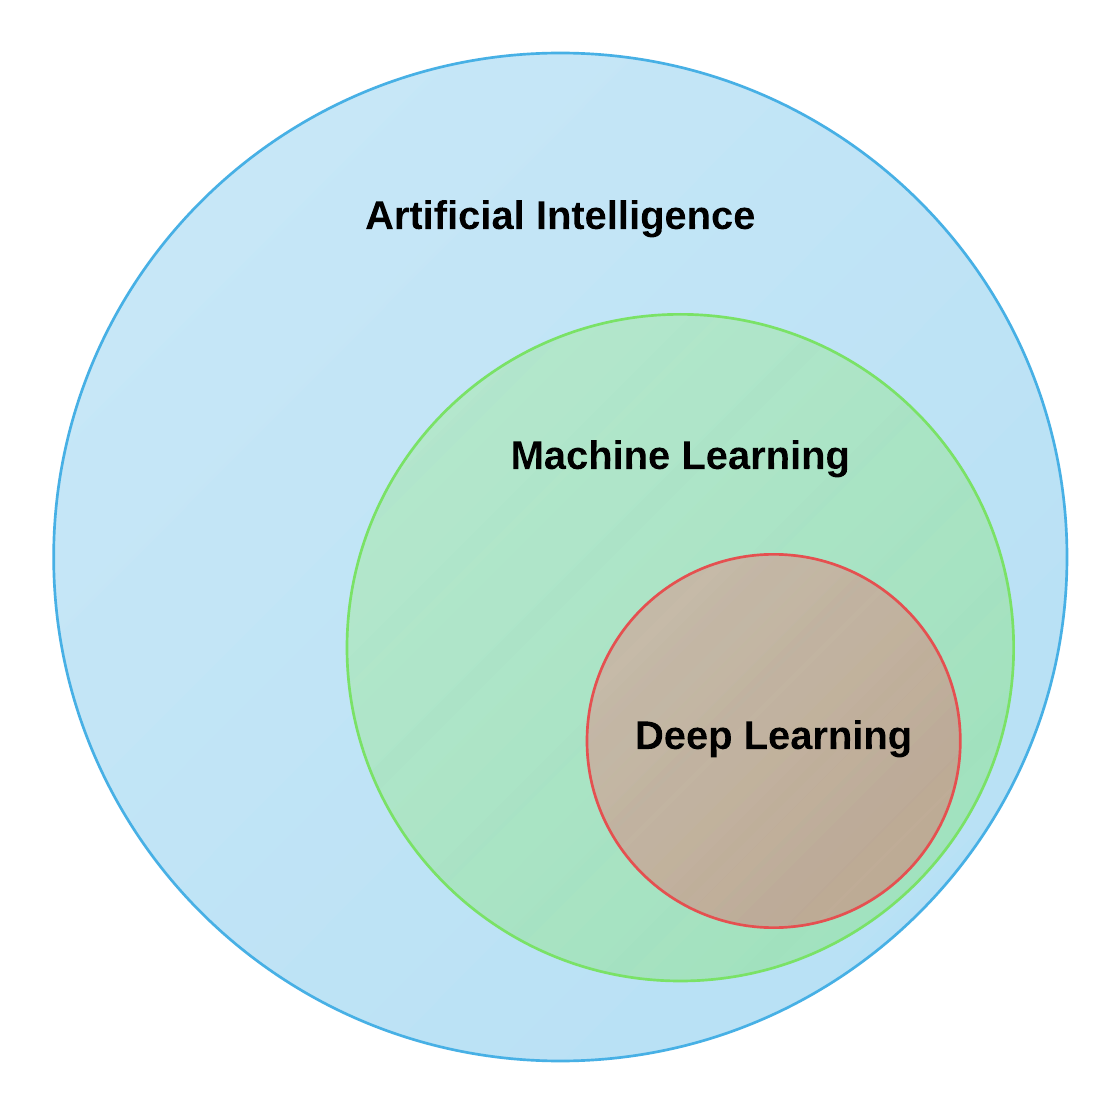
\includegraphics[width=0.5\textwidth]{Pictures/ml_hierarchy.png}
\caption{\label{fig:ml_hierarchy}{}Hierarchy representation of AI, ML and Deep Learning}
\captionsetup{font={footnotesize,bf,it}}
\caption*{Source: https://www.codesofinterest.com/2016/11/difference-artificial-intelligence-machine-learning-deep-learning.html}
\end{figure}


Machine learning models is divided into two types:

\begin{enumerate}
    \item \textbf{Supervised learning} - is the machine learning task of learning a function that maps an input to an output based on example input-output pairs.
    \item \textbf{Unsupervised learning} - is the machine learning tasks that learns from test data that has not been labeled, classified or categorized.
\end{enumerate}




\subsection{Supervised Learning}

Supervised Machine learning models are all about finding appropriate representations for their input data and it requires 3 things:
\begin{enumerate}
    \item \textbf{Input data}. A good data set is the key of creating good Machine Learning model. The input data depends on the problem which the developer want to solve - if the task is speech recognition, then the input data could be sound files converted to the form that computer could proceed, for example: binary. If the task is image tagging, then the data could be a pictures where each pixel is converted to the RGB (red-green-blue) format or HSV (hue-saturation-value) format. The input data depends on the problem and the final goal of the problem. 
    \item \textbf{Output data}. Output data in other words could be called as results of the input data. Supervised machine learning models should know the results of each data input entry point in order to find out a pattern which helps to predict a results. 
    \item \textbf{Validation}. Validation is a way to measure whether the algorithm is doing a good job to determine the distance between the algorithm's current output and its expected output. The validation for supervised machine learning models is split into 2 parts: training data and testing data. Training data is input data and output data which is used for machine learning model training and it from where model learns the patterns of the data which produce certain output. The testing data is used after the machine learning training and from this data the model is evaluated of how successfully it predicted the output results from the input data.
\end{enumerate}


Supervised learning is grouped into two types:

\begin{enumerate}
    \item \textbf{Classification} A classification type is when the output variable is representing a category
    \item \textbf{Regression} A regression type is when the output variable is representing a real value
\end{enumerate}

\subsubsection{Classification}

Classification is the process of predicting the class of given data points. Classes are usually named as a term of \textbf{Labels}. Classification main goal is from given input data points predict an output which would mark a label. Classification predictive modeling: approximating a mapping function (f) from input variables (X) to discrete output variable (y). 


Classification Machine Learning algorithms:

\begin{enumerate}
    \item \textbf{Linear Classifiers} is the statistical classification group of identifying classes of the object's characteristics. A linear classifier methods makes a classification decisions based on the values of a linear combinations of the characteristics. In this paper two linear classifiers would be described: \textit{Logistic Regression} and \textit{Naive Bayes Classifier}
    \begin{enumerate}
        \item \textbf{Logistic Regression}
        \label{sssec:logistic_regression}
        Logistic Regression is a statistical method for analysing a data set in which there are one or more independent variables that determine an measured(outcome) with a dichotomous variable. It predicts the probability of an outcome that have two values. 
        
        The main goal of logistic regression is to find the best fitting model to describe relationship between the dichotomous characteristics of interest and a set of independent variables. 
        
        Logistic regression generates a logistic curve (yellow color) (the Linear and logistic model representation figure \ref{fig:logistic_regression}) which y-axis is limited to values between 0 and 1; [0, 1].
        
        \begin{figure}[H]
            \centering
            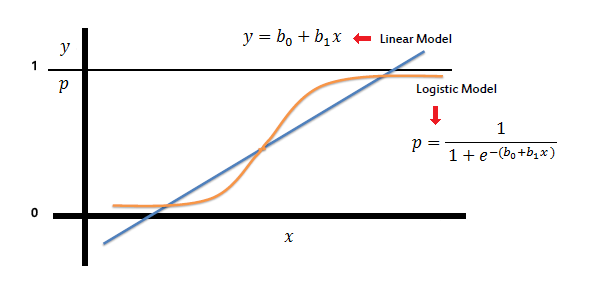
\includegraphics[width=0.8\textwidth]{Pictures/logistic_regression.png}
            \caption{\label{fig:logistic_regression}{} Linear model and Logistic model representation \cite{16}}
        \end{figure}
        
        \textbf{Logistic model} mathematical representation: $p = \frac{1}{1 + e^-(b_{0} + b_{1}x)}$
        
        \textbf{Linear model} mathematical representation: $y = b_{0} + b_{1}x$
        
        \textbf{Logistic regression} could be expressed in the formula:
        
        \begin{equation}
             \frac{p}{1 - p} = \exp{b_{0} + b_{1}x}
        \end{equation}
        \begin{description}
            \item[$p$] Logistic Model 
            \item[$b_{0}$] Logistic regression constant
            \item[$b_{1}$] The slope that defines the steepness of the curve
        \end{description}
        
        \item \textbf{Naive Bayes Classifier}. 
        
        Naive Bayes classifier assumes that the presence of a particular feature in a class is unrelated to the presence of any other feature. Bayes theorem could be expressed in the mathematical equation:
        
        \begin{equation}
                P(A|B) = \frac{P(B|A)P(A)}{P(B)}
        \end{equation}
        \begin{description}
            \item[$A$ and $B$] are events 
            \item[$P(B)$] $\ne 0$
            \item[$P(A | B)$] is a conditional probability: the likelihood of event $A$ occurring given that $B$ is true.
            \item[$P(B | A$] is also a conditional probability: the likelihood of event $B$ occurring given that $A$ is true.
            \item[$P(A)$ and $P(B)$] are the probabilities of observing $A$ and $B$ independently of each other; this is known as the marginal probability
        \end{description}
        
        Naive Bayes \cite{BIB4} is effective in many practical applications including text classification, performance management and medical diagnosis. The effectiveness of Naive Bayes classifier comes from it is presence of feature dependencies: optimality in terms of zero-one loss (classification error) is not necessarily related to the quality of the fit to a probability distribution. 
        
    \end{enumerate}
    \item \textbf{Support Vector Machines(SVM)} 
    
    Support vector machine(SVM) is a discriminative classifier defined by a separating hyperplane. Hyperplane is a line dividing a plane i two parts where in two parts. SVM algorithm main objective is to find a optimal hyperplane in an N-dimensional (N - is the number of features) space that distinctly classifies the data points. 
    
    When using Support Vector Machine it should be considered these parameters:
    
    \begin{itemize}
        \item Input. Set of training pair samples. Call the input sample features $x_{1}, x_{2}...x_{n}$ and the output result y
        \item Output. Set of weights $w$. One for each feature, whose linear combination predicts the value of y
    \end{itemize}
    
    
    
    SVM usage in the real world applications:
    
    \begin{itemize}
        \item Text and Hypertext categorization. SVM method could significantly reduce the need for labeled training instances in both the standard inductive and transductive settings.
        \item Classification of images. SVM achieve higher search accuracy than traditional query refinement schemes
        \item Biological and other sciences. SVM performed good results in classification of proteins schemes or classifying permutation tests.
    \end{itemize}
    
    
    \item \textbf{Decision Trees}
    
    Decision tree are flowchart-like structures that classifies input data points or predict output values given inputs.
    A decision tree is a decision-making device which assigns a probability to each of the possible choices based on the context of the decision: $P(f|h)$, where $f$ is an element of the set of choices and $h$ is the context of the decision. Probability $P(f|h)$ is determined by asking the sequence of questions $q_{1}, q_{2},...,q_{n}$ about the context, where the $ith$ question asked is uniquely determined by the answers to the $i - 1$ previous questions \cite{BIB5}.
    
    
    Decision tree builds classification or regression models in the form of a tree data structure. The data sets is break into smaller subsets. Decisions are represented as nodes and leaf nodes in the tree. 
    
    A decision tree consist of three types of nodes:
    
    \begin{enumerate}
        \item Decision nodes - represented by squares
        \item Chance nodes - represented by circles
        \item End nodes - represented by triangles
    \end{enumerate}
    
    Advantages of Decision trees classification:
    
    \begin{itemize}
        \item Easy to understand and interpret because of the tree structure.
        \item The results could be achieved even with the little data. 
        \item Could determine best, worst and expected values for different scenarios
    \end{itemize}
    
    Disadvantages of Decision trees classification:
    
    \begin{itemize}
        \item It could be unstable. Small changes could imply large changes in the structure of the decision tree
        \item They are often relatively inaccurate comparing with others classification algorithms
        \item Information gain in decision trees is biased in favor of those attributes with more levels
    \end{itemize}
\end{enumerate}

\subsubsection{Regression}

Another type of Machine learning is called Regression. Regression algorithms tries predict a value for an input based on previous information. The main difference of classification type and regression type is that regression main goal is to estimate a value while classification type main goal is to estimate a class of an observation. 

Regression models have the following parameters and variables:

\begin{itemize}
    \item \textbf{The unknown parameters}, denotes as $\beta$, which may represent a scalar or a vector
    \item \textbf{The dependent variable, Y}. This is a main factor that has to be understood and predicted.
    \item \textbf{The independent variables, X}. This is a factor which have an impact on dependent variable
\end{itemize}
A regression model relates Y to a function of X and $\beta$: $Y \approx f(X, \beta)$


Regression Machine Learning algorithms:
\begin{enumerate}
    \item \textbf{Linear Regression}
    
    Linear regression \cite{BIB6} is a technique that analyze the relationships between variables and how they contribute and related to producing a particular outcome. Linear regression establishes a relationship between \textbf{dependent variable (Y)} and \textbf{independent variables (X)} using straight line also known as regression line. 
    
    Linear regression is represented in the formula:
    
    \begin{equation}
     Y = a + b\times X + e
    \end{equation}
    \begin{description}
        \item[Y] Dependent variable 
        \item[X] Independent variables
        \item[a] Intercept
        \item[b] Slope
        \item[e] Error term
    \end{description}
    This equation represents of how Linear Regression method predicts value of target variable on given predictor variables.
    
    Example of the linear regression scatter plot could be seen in the figure \ref{fig:linear_regression}. The black line consists of the predictions, the points are the data and the vertical lines between the points and  the black line represent errors of prediction.
    \begin{figure}[H]
        \centering
        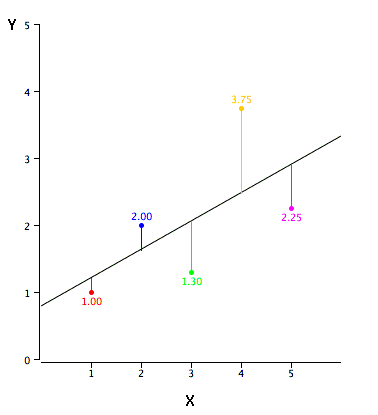
\includegraphics[width=0.55\textwidth]{Pictures/linear_regression.png}
        \caption{\label{fig:linear_regression}{}Scatter plot of the linear regression method \cite{BIB17}}
    \end{figure}
    
    
    Logistic regression \tectbg{properties}:
    
    \begin{itemize}
        \item Linear regression method requires linear relationship between independent variable (Y) and dependent variables X
        \item Linear regression results could be drastically dependent on Outliers. Outliers are the Data points that diverge in a big way from the overall pattern. 
        \item Multicollinearity could increase the variance of the coefficient estimates and make the estimates sensitive to minor changes in the model. Multicollinearity is a statistical process in which predictor variables are correlated.
    \end{itemize}
    
    \textbf{Advantages} of using logistic regression model:
    
    \begin{itemize}
        \item Space complexity of the logistic regression model is low because it needs only to save the weights at the end of training
        \item Good interpretability, simple to understand
        \item Feature importance is generated at the time model building. Dimensionality reduction could be achieved by handling feature selection and by using hyperparameters 
    \end{itemize}
    
    \textbf{Disadvantages} of using logistic regression model:
    
    \begin{itemize}
        \item Multicollinearity should be avoided
        \item Prone to outliers
        \item Linear regression assumes that the data is independent
    \end{itemize}
    
    \item \textbf{Polynomial Regression}
    
    Polynomial Regression method is the relationship between the \textbf{independent variables X } and the \textbf{dependent variable Y} which is modelled as an $nth$ degree polynomial. This method is good for handling non-linearly separable data. This method fits a nonlinear relationship between the value of x and the corresponding conditional mean of Y, denoted as $E(Y|X)$. 
    
    $nth$ degree polynomial regression method could be described in the mathematical formula:
    \begin{equation}
     Y = \beta_{0} + \beta_{1}x + \beta_{2}x^2 + \beta_{3}x^3 + ... + \beta_{n}x^n + e
    \end{equation}
    \begin{description}
        \item[Y] Dependent variable 
        \item[x] Independent variables
        \item[$\beta$] Unknown parameters
        \item[e] Error term
    \end{description}
    
    Polynomial regression properties:
    \begin{itemize}
        \item Otherwise than linear regression, polynomial regression method could model non-linearly seperable data
        \item Full control over the modelling of feature variables
        \item Prone to over fitting if exponents are not selected according to model design.
    \end{itemize}
    
    Polynomial regression have few problems that should be taken to consideration before using this algorithm:
    \begin{enumerate}
        \item When the X values are large, the model could be leaded to the math overflow which could make results inaccurate.
        \item The parameters of the model are intertwined so that lead=s of having covariance and dependency cases between the X values.
    \end{enumerate}
    
    \item \textbf{Ridge Regression}
    
    Ridge regression is a remedial measure taken to alleviate multicollinearity amongst regression predictor variables in a model. By adding a degree of bias to the regression estimates, ridge regression reduces the standart errors rate. 
    
    Ridge regression model formula:
    \begin{equation}
     Y = X\beta + e
    \end{equation}
    \begin{description}
        \item[Y] Dependent variable 
        \item[X] Independent variables
        \item[$\beta$] Regression coefficients to be estimated
        \item[e] Error term
    \end{description}
    
    
    The presence of multicollinearity could be detected in a few ways:
    \begin{itemize}
        \item A regression coefficient is not significant even though variables should be correlated with dependent variable Y
        \item The regression coefficients changes dramatically if X independent variables are added or deleted
        \item X independent variables have high pairwise correlations
    \end{itemize}
    
    Features of ridge regression model:
    \begin{itemize}
        \item The assumption is the same as least squared regression
        \item The value of coefficients does not reach zero
    \end{itemize}
    
    
    \item \textbf{Lasso Regression}
    
    Lasso regression \cite{BIB7} method performs both variable selection and regularization in order to enhance the prediction. Lasso regression and ridge regression are similar methods but lasso regression is using an absolute value bias while ridge regression method is using squared value bias.
    
    The goal of lasso method is to obtain the subset of predictors that minimizes prediction error for a quantitative response variable. This is done by shrinking variables towards zero.
    
    The lasso estimate is defined by formula:
    
    $\beta^{\mathit{lasso}} = argmin \sum_{i=1}^N(y_{i} - \beta{0} - \sum_{j=1}^P x_{ij}\beta_{j})^2$ subject to $\sum_{j=1}^P |\beta_{j}| <= t$ 
    
    Lasso regression translates each coefficient by a constant factor $\lambda$, truncating at zero. This process is called "soft thresholding," and is used in the context of wavelet-based smoothing.
    
    Lasso regression is often an effective technique for shrinkage and feature selection.
    
\end{enumerate}


\subsection{Unsupervised Learning}

Unsupervised machine learning clusters only need to have an input data which would be used for detecting a patterns of the data.  

\subsubsection{Clustering}

Clustering is a task of grouping a set of objects by their data property patterns. Clustering methods are used for identifying similar groups to entities of that group than those of the other groups. Clustering methods are diverse by their types:
\begin{enumerate}
    \item \textbf{Centroid-based}
    
    Clustering model which is related to the notion of similarity is derived by the closeness of a data point to the centroid of the clusters. Using algorithms with this type it is important to know the number of clusters before grouping data.
    
    \item \textbf{Distributed-based}
    
    Clustering model which is based on the notion of how probable is it that all data points in the cluster belong to the same distribution. Distributed-based models tends more suffer from overfitting. 
    
    \item \textbf{Connectivity-based}
    
    Clustering model which is based on the notion that the data points closer in data space exhibit more similarity to each other than the data points lying farther away. This model could be diverse into two approaches:
    \begin{enumerate}
        \item Classifying all data points into separate clusters and then aggregating them as the distance decrease.
        \item All data points are classified as a single cluster and then partitioned as the distance increases.
    \end{enumerate}
    Models are very easy to interpret but lacks scalability for handling big data sets
    
    \item \textbf{Density-based}
    
    Clustering model which is search the data space for areas of varied density of data points in the data space. It isolates various different density regions and assign the data points within these regions in the same cluster.
    
\end{enumerate}


\begin{enumerate} 

    \item \textbf{K-Means Clustering}
    
    K-mean is a centroid model based clustering algorithm which the main goal is to partition the inputs into sets $S1,...,S_{k}$ in a way that minimizes the total sum of squared distances from each point to the mean of its assigned cluster. $k$ representing the number of clusters. 
    
    K-means \cite{BIB8} clustering abstract algorithm:
    
    \begin{enumerate}
        \item Decide on a value for K, the number of clusters
        \item Initialize the K cluster centers 
        \item Decide the class memberships of the N objects by assigning them to the nearest cluster center
        \item Re-estimate the K cluster centers, by assuming the memberships found above are correct
        \item Repeat c and d until none of the N objects changed membership in the last iteration
    \end{enumerate}
    
    \textbf{Advantages} of K-mean clustering :
    \begin{itemize}
        \item K-mean clustering is fast. Computing the distances between points and group centers requires few computations. The linear complexity of the algorithm is \textbf{O(n)}
        \item An instance could move to another cluster when the centroids are recomputed
        \item Converges to local minimum of within-cluster squared error
    \end{itemize}
    
    
    \textbf{Disadvantages} of K-mean clustering:
    \begin{itemize}
        \item The exact number of clustering groups/classes should be known before using k-means clustering algorithm 
        \item K-means starts with a random choice of cluster centers and it could perform different results for each algorithm run
        \item The order of the data has an impact to the final results
        \item Sensitive to outliers
        \item Detects spherical clusters only
    \end{itemize}
    
    
    \item \textbf{Mean-Shift Clustering}
    
    Mean-shift \cite{BIB9} clustering algorithm is a non parametric clustering technique which does not require prior knowledge of the number of clusters and does not constrain the shape of the clusters. 
    
    
    \begin{equation}
        K(x) = 
        \left \{
          \begin{tabular}{ccc}
          1 if ||x|| <= \lambda \\
          0 if ||x|| > \lambda 
          \end{tabular}
        \right \}
    \end{equation}
    \begin{description}
         Let data be a finite set $S$ embedded in the n-dimensional Euclidean space, $X$. Let $K$ be a flat kernel that is the characteristic function of the $\lambda$-ball in $X$
    \end{description}
    The sample mean at x \in X is:
    
    \begin{equation}
        m(x) = \frac{\Sigma_{s \in S} K(s-x)s}{\Sigma_{s \in S} K(s-x)}
    \end{equation}
    
    The difference $m(x) - x$ is called \textit{mean shift}. In each iteration of the algorithm, $s \Leftarrow m(s)$ is performed for all $s \in S$ simultaneously. The mean shift vector always points toward the direction of the maximum increase in the density.
    
    Mean-shift clustering abstract algorithm:
    \begin{enumerate}
        \item Circular sliding window centered at a randomly selected point $C$ and having radius $r$ as the kernel. 
        \item At every iteration the sliding window is shifted towards regions of higher density by shifting the center points to the mean of the points withing the window while there is direction at which a shift can accommodate more points inside the kernel
        \item  This process of steps (a) and (b) is done with many sliding windows until all points lie within a window.
    \end{enumerate}
    
    
    \textbf{Advantages} of Mean-Shift clustering:
    \begin{itemize}
        \item Model free - does not assume any prior shape on data clusters
        \item It requires single parameter of window size $h$
        \item Robust to outliers
    \end{itemize}
    
    \textbf{Disadvantages} of Mean-Shift clustering:
    \begin{itemize}
        \item Results depends on window size
        \item Window size selection is not trivial
        \item Computationally expensive
        \item Does not scale well with dimension of feature space
    \end{itemize}
    
    \item \textbf{Density-Based Spatial Clustering of Applications with Noise (DBSCAN)}
    
    Density-Based Spatial Clustering of Applications with Noise (DBSCAN) is a density based clustering algorithm. Given a set of points in some space, it groups together points that are closely packed together, marking as outliers points that lie alone in low-density regions. Overall average complexity of DBSCAN clusetering algorithm is \textbf{O(log n)}.
    
    DBSCAN abstract algorithm:
    \begin{enumerate}
        \item Find the points in the $\epsilon$ neighborhood of every point, and identify the core points with more than $minPts$ neighbors
        \item Find the connected components of core points on the neighbor graph, ignoring all non-core points
        \item Assign each non-core point to a nearby cluster if the cluster is an $\epsilon$ neighbor, otherwise assign it to noise
    \end{enumerate}
    
    
    \textbf{Parameters}  of DBSCAN clustering algorithm:
    \begin{itemize}
        \item $MinPoints$: The minimum number of points to form a dense region 
        \item $\epsilon$: The minimum distance between two points. The points are considered neighbors if the distance between two points is lower or equal to $\epsilon$ value
    \end{itemize}
    
    
    \textbf{Advantages} of DBSCAN clustering algorithm:
    \begin{itemize}
        \item DBSCAN does not require one to specify the number of clusters in the data
        \item DBSCAN can find arbitrarily shaped clusters
        \item DBSCAN has a notion of noise, and is robust to outliers
        \item DBSCAN requires just two parameters and is mostly insensitive to the ordering of the points in the database
        \item DBSCAN is designed for use with databases that can accelerate region queries, e.g. using an R* tree
    \end{itemize}
    
    
    \textbf{Disadvantages} of DBSCAN clustering algorithm:
    \begin{itemize}
        \item DBSCAN is not entirely deterministic: border points that are reachable from more than one cluster can be part of either cluster, depending on the order the data are processed
        \item The results of DBSCAN model depends on the distance measure
        \item DBSCAN cannot cluster data sets well with large differences in densities
        \item Choosing a meaningfull distance treshhold $\epilepson$ could be difficult if the data is not proper for this algorithm
    \end{itemize}
    
    
    
    \item \textbf{Expectation–Maximization (EM) Clustering}
    
    The Expectation–Maximization clustering algorithm is an iterative method to find maximum likelihood or maximum a posteriori (MAP) which computes probabilities of cluster memberships based on one or more probability distributions. The goal of the EM clustering algorithm is to maximize the overall probability or likelihood of the data.
    
    
    The EM algorithm seeks to find the MLE of the marginal likelihood by iteratively applying these two steps:
    \begin{enumerate}
        \item Expectation step (E step): Define $\Theta(\theta|\theta^{(t)})$ as the expected value of the log likelihood function of $theta$, with respect to the current conditional distribution of $Z$  given $X$  and the current estimates of the parameters $\theta^{(t)$:
        \begin{equation}
            \Theta(\theta|\theta^{(t)}) = E_{Z|X_{1}\theta^{(t)}}[\log L(\Theta;X;Z)]
        \end{equation}
        \item Maximization step (M step): Find the parameters that maximize this quantity:
        \begin{equation}
            \theta^{(t+1)} = arg max_\theta \Theta(\theta|\theta^{(t)}
        \end{equation}
    \end{enumerate}
    
    \begin{description}
        \item [X] Observed data
        \item [Z] a set of unobserved latent data or missing values $Z$ 
        \item [$\theta$] a vector of unknown parameters
        \item [$L(\theta,X, Z)$] likelihood function
    \end{description}
    
    
    Expectation–Maximization abstract algorithm:
    \begin{enumerate}
        \item Initialize the parameters $\theta$ to some random values
        \item Compute the probability of each possible value of $Z$, given $\theta$
        \item Use the just-computed values of $Z$  to compute a better estimate for the parameters $\theta$
        \item Iterate steps (b) and (c) until convergence
    \end{enumerate}
    
    
    \textbf{Advantages} of Expectation–Maximization clustering algorithm:
    \begin{itemize}
        \item Likelihood is guaranteed to increase for each iteration
        \item Is a derivative-free optimizer
        \item Is fast if analytical expressions for the M-step are available
        \item Parameter constraints are often dealt with implicitly
    \end{itemize}
    
    
    
    \textbf{Disadvantages} of Expectation–Maximization clustering algorithm:
    \begin{itemize}
        \item Requires both forward and backward probabilities
        \item Significant implementational effort required compared to numerical optimization
        \item I Convergence may be slow if analytical expressions for the M-step are not available since numerical optimization must be applied
        \item Hessian must be calculated manually
    \end{itemize}
    
    
    
    \item \textbf{Hierarchical Clustering}
    
   Hierarchical clustering \cite{BIB10} is a method of cluster analysis which seeks to build a hierarchy of clusters. Hierarchical clustering algorithm run once and create a dendrogram which is a tree structure containing a k-block set partition for each value of k between 1 and n, where n is the number of data points to cluster allowing the user to choose a particular clustering. 
   
   
   Hierarchical clustering consist of two types:
   \begin{enumerate}
       \item \textbf{Agglomerative}:  This is a "bottom-up" approach: each observation starts in its own cluster, and pairs of clusters are merged as one moves up the hierarchy. Bottom-up algorithms treat each data point as a single cluster at the outset and then successively merge  pairs of clusters until all clusters have been merged into a single cluster that contains all data points. The time complexity of this method is $O(n^3)$.
       \item \textbf{Divisive}: This is a "top-down" approach: all observations start in one cluster, and splits are performed recursively as one moves down the hierarchy. Divisive clustering complexity is $O(2^n)$. 
   \end{enumerate}
    
    
    Agglomerative Hierarchical clustering abstract algorithm \cite{BIB11}:
    \begin{enumerate}
        \item Compute the similarity between all the pairs of clusters
        \item Combine the foremost similar two clusters
        \item Update the similarity matrix to replicate the pairwise similarity between the new cluster and the original clusters
        \item Repeat steps b and c until only a single cluster remains
    \end{enumerate}
    
    
    \textbf{Advantages} of Hierarchical clustering algorithms:
    \begin{itemize}
        \item Hierarchical clustering does not require us to specify the number of clusters
        \item Algorithm is not sensitive to the choice of distance metric
    \end{itemize}
    
    
    \textbf{Disadvantages} of Hierarchical clustering algorithms:
    \begin{itemize}
        \item Sensitivity to noise and outliers
        \item Breaking large clusters
        \item Difficulty handling different sized clusters and convex shapes
    \end{itemize}
    
\end{enumerate}


\subsubsection{Dimensionality reduction}

Dimensionality reduction \cite{BIB13} is the transformation of high-dimensional data into a meaningful representation of reduced imensionality.Ideally, the reduced representation should have a dimensionality that corresponds to the intrinsic dimensionality of the data. The intrinsic dimensionality of data is the minimum number of parameters needed to account for the observed properties of the data.


The problem of dimeansionality reduction could be defined as follows: Data set is represented in a $n$ x $D$ matrix $X$ consisting of $n$ datavectors $x_{i} (i \in {1, 2, ..., n})$ ) with dimensionality $D$. The data set has intrinsic dimensionality $d (where d < D)$, in mathematical terms, intrinsic dimensionality means that the points in data set $X$ are
lying on or near a manifold with dimensionality $d$ that is embedded in the D-dimensional space. 
Dimensionality reduction techniques transform dataset $X$ with dimensionality $D$ into a new data set $Y$ with dimensionality $d$, while retaining the geometry of the data as much as possible. High-dimensional data point is denoted by $x_{i}$ , where $x_{i}$ is the $i$th row of the D-dimensional data matrix $X$. The low-dimensional counterpart of $x_{i}$ is denoted by $y_{i}$ , where $y_{i}$ is the $i$th row of the d-dimensional data matrix $Y$. The data set $X$ is assumed as a zero-mean.


There are two components of dimensionality reduction:
\begin{enumerate}
    \item \textbf{Feature selection}. The subset of the original set of variables are found to get a smaller subset which could be used to model the problem. This component is divided into three separate parts:
    \begin{enumerate}
        \item \textit{Filter}. Filter out features with small potential to predict outputs. Filter operation could be expressed in mathematical representation:
        \begin{enumerate}
            \item Let $\Phi$ be a current set of features
            \item Removing feature $\phi_}k}(x)$ is possible only when:
            \begin{equation}
                \Tilde{P}(y|\Phi|\phi_{k}) \approx \Tilde{P}(y|\Phi)
            \end{equation}
            For all values of $\phi_{k}, y$
        \end{enumerate}
       
        \item \textit{Wrapper}. Select features that directly optimize the accuracy of the classifier
        \item \textit{Embedded}. Features are selected to add or be removed while building the model based on the prediction errors
    \end{enumerate}
    \item \textbf{Feature extraction}. Reduces the data in a high dimensional space to a lower dimension space
\end{enumerate}


\textbf{Advantages} of Dimensionality Reduction:
\begin{itemize}
    \item Improves performance in data compression
    \item Reduces computation time
    \item Removes redundant features
    \item Hence reduced storage space
\end{itemize}


\textbf{Disadvantages} of Dimensionality Reduction:
\begin{itemize}
    \item It may lead to some amount of data loss.
\end{itemize}


\begin{enumerate}
    \item \textbf{Principal Component Analysis (PCA)}
    
    Principal component analysis (PCA) is a statistical procedure that uses an orthogonal transformation to convert a set of observations of possibly correlated variables into a set of values of linearly uncorrelated variables called principal components. PCA is a linear transformation of $d$ dimensional input $x$ to $M$ dimensional feature vector $z$ such that under which the retained variance is maximal. It is also considered as the linear projection for which the sum of squares reconstruction cost is minimized. 
    
    
    \textbf{Goals} of Principal Component Analysis (PCA):
    \begin{itemize}
        \item Simplification
        \item Data reduction
        \item Outlier Detection
        \item Variable selection
        \item Classification
        \item Prediction
        \item Unmixing
    \end{itemize}
    
    
    Many of the goals of PCA are concerned with finding relationships between objects. PCA estimates the correlation structure of the variables. The importance of a variable in a PC model is indicated by the size of its residual variance. 

    
    PCA \cite{BIB14} in matrix form is the least squares model:
    \begin{equation}
        X = 1\Tilde{x} + TP' + E
    \end{equation}
    \begin{description}
        \item [$\Tilde{x}$] Mean vector which is included in the model formulation
        \item [P'] Projection matrix. It is also called loading vector
        \item [T] Object coordinates in the plane. It is also called scoring vectors
        \item [X] The projection
        \item [E] The deviations between projections and the original coordinates are termed the residuals.
    \end{description}
    
    
    \item \textbf{Linear Discriminant Analysis (LDA)}
    
    Linear Discriminant Analysis (LDA) \cite{BIB15} is a method to find a linear combination of features that characterizes or separates two or more classes of objects or events. 
    
    Given a data matrix $A \in \R^{N×n}$, classical LDA aims to find a transformation $G \in \R^{N×t}$ that maps each column $a_{i}$ of $A$, for $1 ≤ i ≤ n$, in the N-dimensional space to a vector $b_{i}$ in the $\iota$-dimensional space. That is $G$ : $a_{i} \in \R \Leftarrow b_{i} = G^T a_{i} \in \R^{\iota} (\iota < N)$. Equivalently, classical LDA aims to find a vector space $G$ spanned by {g$_{i}}^{\iotai}_{i=1}$}, where $G = [g_{1},..., g_{\iota}]$, such that each $a_{i}$ is projected onto $G$ by $(g^{T}_{1} · a_{i},..., g^{T} · a_{i})T \in \R^{\iota}$.
    
    
    Assume that the original data in $A$ is partitioned into $k$ classes as $A = {\Pi_{1}, ... , \Pi_{k}}$, where $\Pi_{i}$ contains $n_{i}$ data points from the $i$th class, and $\sum\limits{i=1}^{k} n_{i} = n$. Classical LDA aims to find the optimal transformation $G$ such that the class structure of the original high-dimensional space is preserved in the low-dimensional space. In general, if each class is tightly grouped, but well separated from the other classes, the quality of the cluster is considered to be high. In discriminant analysis, two scatter matrices, called within-class ($S_{w}$) and between-class ($S_{b}$) matrices, are defined to quantify the quality of the cluster, as follows [4]: $S_{w} = \sum\limits{i=1}^{k} \sum\limits{x \in \Pi_{i}} (x − m_{i})(x − m_{i})T$, and $S_{b} = \sum\limits{i=1}^{k} n_{i}(m_{i} − m)(m_{i} − m)T$, where $m_{i} = \frac{1}{n_{i}} \sum\limits{x \in \Pi_{i}} x$ is the mean of the $i$th class, and $m = \frac{1}{n}\sum\limits{i=1}^{k} \sum\limits{x \in \Pi|{i}} x$ is the global mean. 
    
    Notation:
    \begin{description}
        \item [$n$] number of instances in the data set
        \item [$k$] number of classes in the data set
        \item [$A_{i}$] $i$th instance in matrix representation
        \item [$a_{i}$] $i$th instance in vectors representation
        \item [$r$] r number of rows in $A_{i}$
        \item [$c$] number of columns in $A_{i}$
        \item [$N$] dimension of $a_{i} (N = r ∗ c)$
        \item [$\Pi$] $j$th class in the data set
        \item [$L$] transformation matrix (left) by Two-Dimensional Linear Discriminant Analysis
        \item [$R$] transformation matrix (right) by Two-Dimensional Linear Discriminant Analysis
        \item [$I$] number of iterations in Two-Dimensional Linear Discriminant Analysis
        \item [$B_{i}$] reduced representation of $A_{i}$ by Two-Dimensional Linear Discriminant Analysis
        \item [$\iota_{1}$] number of rows in $B_{i}$
        \item [$\iota_{2}$] number of columns in $B_{i}$
    \end{description}
    
    
    The goal of Linear Discriminant Analysis (LDA) is to project a data set onto a lower-dimensional space with good class-separability in order avoid overfitting and also reduce computational costs.
    
    
    \textbf{Pseudo algorithm} for using LDA approach:
    \begin{enumerate}
        \item Compute the $d$-dimensional mean vectors for the different classes from the data set
        \item Compute the scatter matrices
        \item Compute the eigenvectors ($e_{1},e_{2},...,e{d}$) and corresponding eigenvalues ($\lambda_{1},\lambda_{2},...,\lambda_{d}$) for the scatter matrices
        \item Sort the eigenvectors by decreasing eigenvalues and choose $k$ eigenvectors with the largest eigenvalues to form a $d$×$k$ dimensional matrix $W$
        \item Use $d$×$k$ eigenvector matrix to transform the samples onto the new subspace. This can be summarized by the matrix multiplication: $Y$=$X$×$W$, where 
        \begin{description}
            \item [X] is a $n$×$d$-dimensional matrix representing the $n$ samples
            \item [Y] are the transformed $n$×$k$-dimensional samples in the new subspace
        \end{description}
    \end{enumerate}
    
\end{enumerate}


\subsubsection{Association analysis}

Association analysis is a method which is useful for discovering relationships hidden in large data sets. The uncovered relationships can be represented in the form of sets of items present in many transactions, which are known as \textbf{association rules} that represents relationships between two item sets. Association rule mining finds all rules in the database that satisfy some minimum support and minimum confidence constraints.

One of the real life examples in where association rules could be used is two items expression:

\textbf{Olives} \rightarrow \textbf{Wine}

The rule suggest a relationship between olives usage with wine because olives is well know a good pair with wine. 

An \textbf{association rule} \cite{BIB12} is an implication expression of the form $X \rightarrow Y$ , where $X$ and $Y$ are disjoint item sets, i.e., $X ∩ Y = ∅$. The strength of an association rule can be measured in terms of its support and confidence. Support determines how often a rule is applicable to a given data set, while confidence determines how frequently items in $Y$ appear in transactions that contain $X$. These metrics has an formal definitions:

\begin{equation}
    Support, s(x \rightarrow Y) = \frac{\delta(X \cup Y)}{N}
\end{equation}
\begin{equation}
    Confidence, c(x \rightarrow Y) = \frac{\delta(X \cup Y)}{\delta(X)}
\end{equation}

\subsection{Machine Learning models evaluation}
Machine Learning models performance could be evaluated of how well they are classifying websites categories. Evaluation scores is a first level indicator which lets to know of Machine Learning capabilities of predicting categories according to the primary training features data sets.

Machine Learning models could predict website categories when training features set are fitted into model. After that model is fed with training features set and it outputs prediction set of predicted categories of websites. These predicted categories are compared with training labels set. Models predictions set and training labels set allows to generate evaluation scores and analysis of how well model is trained to predict categories of websites. 

Calculating models predictions scores, there are 4 special terms which appears in the formulas:
\begin{itemize}
    \item \textbf{True Positives (TP)} - is an outcome where the model correctly predicts the positive class. Example of true positive condition: \textit{Person with disease was diagnosed a disease}.
    \item \textbf{True Negatives (TN)} - is a true negative is an outcome where the model correctly predicts the negative class. Example of true negative condition: \textit{Person with no disease was not diagnosed a disease}.
    \item \textbf{False Positives (FP)} - is a result that indicates a given condition exists, when it does not. A false positive error is a type I error where the test is checking a single condition, and wrongly gives an affirmative decision.  Example of false positive condition:: \textit{Healthy person was diagnosed with a specific disease}. 
    \item \textbf{False Negatives (FN)} - is a test result that indicates that a condition does not hold, while in fact it does. A false negative error is a type II error occurring in a test where a single condition is checked for and the result of the test is erroneously that the condition is absent.  Example of false negative condition:: \texit{Person with disease was diagnosed with no disease}.
\end{itemize}

There are several methods to evaluate machine learning models :
\begin{enumerate}
    
    \item \textbf{Accuracy score}
    
    Classification accuracy is the number of correct predictions made as a ratio of all predictions made.
    
    The accuracy score is calculated by formula:
    \begin{equation}
        Accuracy = \frac{TP + TN}{TP + TN + FP + FN}
    \end{equation}
    
    \item \textbf{Recall score}
    
    Recall score is the number of true positives divided by the number of true positives plus the number of false negatives.
    
    The recall score is calculated by formula:
    \begin{equation}
        Recall = \frac{TP}{TP + FN}
    \end{equation}
    
    \item \textbf{Precision score}
    
    Precision evaluation method determines of how precise/accurate machine learning model of how many positives predictions have been predicted of total predictions. Precision score is calculated by formula:
    \begin{equation}
        Precision = \frac{TP}{\mathit{TP} + \mathit{FP}}
    \end{equation}
    
    Precision is a good measure to determine, when the costs of False Positive is high. 
    
    
    \item \textbf{F1 score}
    
    F1 score is the harmonic mean of precision and recall taking both metrics into account. F1 score is calculated by formula:
    \begin{equation}
        F1 = 2 * \frac{Precision * Recall}{Precision + Recall}
    \end{equation}    
    \item \textbf{Confusion Matrix}
    
    A confusion matrix is a technique for summarizing the performance of a classification algorithm. Confusion matrix is a method to better understand the performance of classification models. It is a summary of of prediction results on a classification models: The number of correct and incorrect predictions are summarized with count values and broken down by each class. This is the key to the confusion matrix.
    
    

\end{enumerate}


\section{Implementation}
The implementation program main goal is to detect URL category of URL page HTML content. It is made by combining Natural Language Processing(NLP) and Machine Learning(ML) which are described in the Approach sections(links). 

The implementation part consists of these sections:

\begin{enumerate}
    \item {The data set of URLs list}
    \item {Data set creation using NLP techniques}
    \item {Data preprocessing}
    \item {Data training using ML techniques}
    \item {Results and conclusions}
\end{enumerate}


The goal of the project is to solve the URL categorization task using a supervised classification algorithm and using a database with a large number of categorized websites. A supervised classified
should be learned to predict the category a web page belongs to.



\subsection{Data preprocessing}

The one of the most important things solving Machine Learning kind of problems is valid data set source which is required for creating testing and training data sets which are required for training and testing Machine Learning model.

The data set of this problem is available at \href{https://www.figure-eight.com/data-for-everyone/}{Data For Everyone data set lists}. The data set contains 31086 different URLs with 81 attributes. Since the data set has a lot of attributes and few of them will be used in the implementation project, attributes could be represented in this kind of manner:
\begin{itemize}
    \item \textit{unit id}
    \item \textit{golden}
    \item \textit{unit state}
    \item \textit{trusted judgments}
    \item \textit{trusted judgments at}
    \item \textit{main category}
    \item \textit{main category:confidence}
    \item \textit{sub category: Each category}
    \item \textit{sub category: Each category:confidence}
    \item \textit{url}
\end{itemize}

It is an enormous data set and all attributes is barely useful for the implementation problem, the size of data set attribute should be reduced. For the implementation part problem, 3 attributes must be extracted, other attributes should be excluded since they have no impact to the ML model creation. 

List of attributes that are extracted for implementation part:
\begin{enumerate}
    \item \textbf{main\_category} : Attribute describes URL main category.
    \item \textbf{main\_category:confidence} : Attribute describes a probability of accuracy of the URL main category. Since URLs could have a lot of sub-categories it provides information about the most likely main category.
    \item \textbf{url} : Attribute provides URL address of the web page.
\end{enumerate}

\label{sec:categoriesSet}
The data set consist of 25 categories:
\begin{table}[H]
    \begin{tabular}{| l | l | l | l |}
        \hline
         Adult & Finance & News \& Media & Arts \& Entertainment   \\ \hline
         Food \& Drink & People \& Society & Automotive & Gambling   \\ \hline
         Pets \& Animals & Beauty \& Fitness & Games & Reference   \\ \hline
         Books \& Literature & Health & Science & Business \& Industry  \\ \hline
         Home \& Garden & Shopping & Career \& Education & Internet \& Telecom  \\ \hline
         Sports & Computer \& Electronics & Law \& Government & Travel\\ \hline
    \end{tabular}
\captionof{table}{The table of all possible categories} 
\label{table: categories_table}
\end{table}


The primary data is not enough to determine in which category given URL belongs it needs some data preprocessing in order to make a vector and label set for Machine Learning algorithms. 

Data preprocessing consist of 6 major steps:
\begin{enumerate}
    \item Website scraping and text parsing
    \item Text tokenization
    \item Removing stop words and normalizing text
    \item Website language determination
    \item Words frequency
    \item Chunk words
\end{enumerate}

The whole image of the processes could be seen in the figure \ref{fig:dataset_creation}:
\begin{figure}[H]
\centering
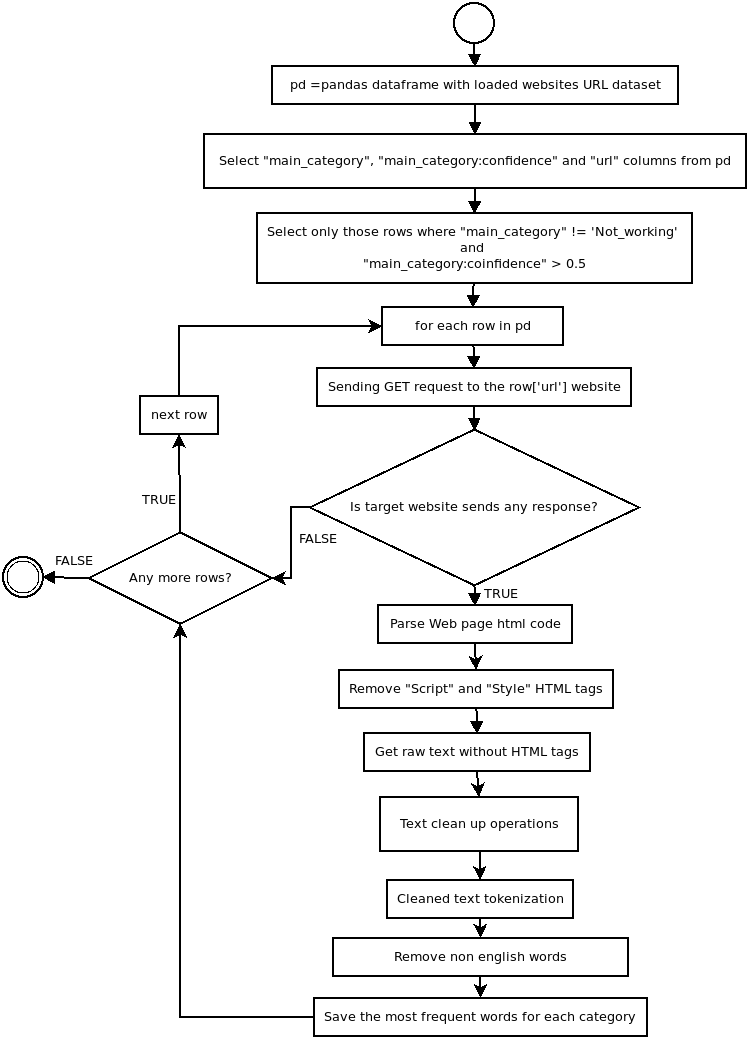
\includegraphics[width=0.8\textwidth]{Pictures/dataset_creation.png}
\caption{\label{fig:dataset_creation}{}Diagram of operations in the data preprocessing}
\end{figure}

Figure \ref{fig:dataset_creation} represents steps that performs data downloading, data filtering and data clean up operations. Since there are a lot of process in this algorithm, in this implementation part each process would be described separately in more depth. 

\subsubsection{Website scraping and text parsing}

The first process is to analyze website and download its content. Every website is build up using HTML language as a core code and the additional design and performance features are added using CSS and JavaScript tools.

The category of the website determines website content. The content is written in the HTML programming language using special tags for displaying information for a user. The main goal of this process is to download the content and parse only necessary text which would be useful for this project. 

This section consist of two parts:
\begin{enumerate}
    \item \textbf{Downloading website content}
    
    Each website content is downloaded by sending GET request using python library \href{https://docs.python.org/3/library/urllib.html}{Urlib}. This library allows to perform GET request to the website and tracks it response.
    
    The expected response from the website is HTML code including Cascading Style Sheets(CSS) and JavaScript(JS) codes. However some websites have security features from scrapping programs, so it is not always possible to get content information from the website. Each website could see the program request header and determine that the request is not performed by the ordinary user and in this case some websites do not respond with the proper information.
    
    Before sending an GET request to the website, the request headers properties are changed to the more likely normal browser properties in order to prevent websites for returning inappropriate response with the HTML content. Also the timeout of the request headers is set to the 15 seconds in order to make some additional time for website response. 
    
    The website is skipped if it is not responding to the GET request
    
    \item \textbf{Website content text parsing}
    
    Website response contains HTML code where the necessary text is stored. There are no need to store text within HTML tags so the other step is to leave only text by excluding HTML tags. This is made by using python library \href{https://pypi.org/project/beautifulsoup4/}{beautifulsoup}. Text parsing consist of these steps:
    \begin{enumerate}
        \item Parse text into beautiful soup object for text filtering and manipulation properties
        \item Filter out CSS and JavaScript content. CSS language is additional tool for improving HTML design which is marked with \textit{<style>} HTML tag and JavaScript is programming language for website behaviour which is marked with \textit{<script>} HTML tag. These elements usually do not contain any useful information so these HTML tags are removed by using beutiful soup function \textit{decompose()}
        \item Text of remain HTML code is extracted by removing HTML tags. HTML tags are removed by using beautiful soup function \textit{get\_text()}
        \item New lines symbols \textit{\n} are removed from the text
        \item The extracted text is stripped in order to remove empty symbols in the text
        \item Every word is joined to the text string by a new line
    \end{enumerate}
\end{enumerate}


\subsubsection{Text tokenization}

The plain text of the website content is not proper format for this project because there is a small probability that the text would be the same among different websites with the same category. However the probability is much bigger that the separated words would more likely to be similar among other website with the same category. This is the reason why the text should be split up to the tokens which would perform plays an important role into project development. 

The parsed text of the website is split up into tokens by using regular expression word tokenizer. Regular expression tokenizer is expressed by this regular expression query: 


\verb/((?<=[^\w\s])\w(?=[^\w\s])|(\W))+$/.

Regular expression symbols explanation:
\begin{description}
    \item \verb/?/ A question mark matches zero or one of the preceding character, class, or sub-pattern. 
    \item \verb/<?=/ Is a positive lookahead, a type of zero-width assertion. What it's saying is that the captured match must be followed by whatever is within the parentheses but that part isn't captured.
    \item \verb/\/ Classes of characters: The square brackets enclose a list or range of characters (or both).
    \item \verb/^/ May appear at the beginning of a pattern to require the match to occur at the very beginning of a line.
    \item \verb/\W/ Matches any single "word" character, namely alphanumeric or underscore.
    \item \verb/\s/ Matches any single white space character, mainly space, tab, and newline (`r and `n). Conversely, capital \S means "any non-white space character". 
    \item + A plus sign matches one or more of the preceding character, class, or sub-pattern.
\end{description}
This regular expression is passed to the \href{https://www.nltk.org/_modules/nltk/tokenize/regexp.html}{nltk python library RegexpTokenizer} function giving an plain text as parameter and it converts plain website text into tokens.

When the text is tokenized, each token word is converted to the lower case. This is made because upper and lower cases have different ASCII codes, so the computer the same words with different ASCII codes treats words as different despite that the words have the same meaning.

\subsubsection{Removing stop words and normalizing text}

\label{sec:stopWords}

Tokens of the website text contains a lot of words, but this does not mean that all the words are proper to use for creating a Machine Learning model. At this point tokens could consist of stop words and random symbols and word could be written in a different grammar forms(singular and plural). These words take a lot of volume in the data, so the volume should be reduced by performing text normalization operations such as \textbf{Removing stop words} and \textbf{Words lemmatization}.


The full image of this process could be seen in a implementation code flowchart figure(\ref{fig:stop_lemma_text}):
\begin{figure}[H]
    \centering
    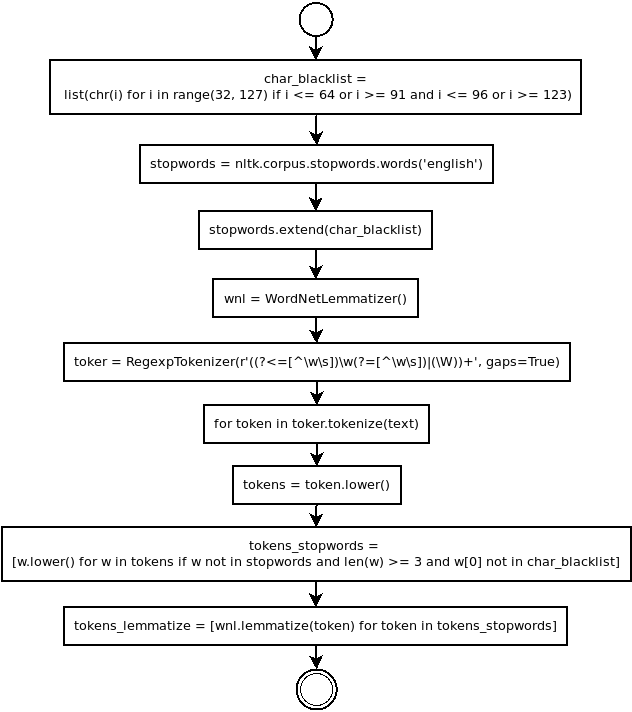
\includegraphics[width=1\textwidth]{Pictures/stop_lemma_text.png}
    \caption{\label{fig:stop_lemma_text}{} An algorithm for processing stop words exclusion and words lemmatization }
\end{figure}

\begin{enumerate}
    \item \textbf{Removing stop words}
    
    Stop words are considered to be common words in a human language which do not provide lots of information by using itself. Tokens contains a list of words that means that they are not connected to the each other and some words by itself do not provides useful information. This is the reason why these words should be removed from the token list because they could confuse the model since most likely every category would contain the same set of words (stop words).
    
    English language is considered of having around 180 stop words. The stop words list database could be found on the internet but for this project \href{https://www.nltk.org/book/ch02.html}{stopwords.words('english')} function which contains 179 commonly used english language stop words. 
    
    
    The main goal of this process is to make sure that the words in the tokens would be meaningful as much as possible, so the additional rules of stop words determination is added. The words with length less than 3 is also considered as as stop words because in english language there are not many words that would contains meaningful information. This is done in order to prevent random symbols that is not determined as words in the english language. The list of these kind of random symbols is made by using \href{http://www.asciitable.com/ASCII} {ASCII(American Standard Code for Information Interchange) table}. The symbols which are in the range of the ASCII table of: [32 : 64], [91 : 96], [123:127] are considered as the stop words. The integer numbers from the range are generated and they are converted to the char symbols that are saved into the list. The list of these symbols are:
    
    ' , !, ", #, \$, \%, \&, \', \(, \), \*, \+, ,, -, ., /, 0, 1, 2, 3, 4, 5, 6, 7, 8, 9, :, ;, <, =, >, ?, @, [, \, ], \^, \_, `, {, |, }, ~'
    
    
    When the stop words list is generated then it is possible to filter out stop words from the tokens. The pseudo algorithm of stop words elimination from the token list:
    \begin{enumerate}
        \item Each word from the token list is iterated
        \item If word is in stop words list then this word is excluded from the token list else the word remains in the token list
    \end{enumerate}
        
    \item \textbf{Words lemmatization}
    
    Words lemmatization  in linguistics is the process of grouping together the inflected forms of a word so they can be analyse as a single item, identified by the word's lemma, or dictionary form. English words grammatically could have 2 forms - singular and plural form. The words core meaning of singular and plural forms remains the same, but the program would treat them as totally different words. The words form is not important for this project problem, so the goal of this process is to have one form for all words that these words would be treated equally according to their core meaning. 
    
    The words lemmatization is done by using english words dictionary of singular and plural forms. The dictionary is build in in the \href{https://www.nltk.org/_modules/nltk/stem/wordnet.html}{nltk python library WordNetLemmatizer} function. The function takes a word as argument and returns a singular form of the word, for example:
    
    
        $children \longrightarrow child$
        
        $word  \longrightarrow words$
    
        $word \longrightarrow word$
        
        
    The examples demonstrates how words forms are converted. The rules of word lemmatization:
    \begin{itemize}
        \item If input word is in a \textbf{singular} form, then output would be an input word in a \textbf{singular} form
        \item If input word is in a \textbf{plural} form, then output would be an input word in \textbf{singular} form
    \end{itemize}
\end{enumerate}

\subsubsection{Website language determination}

There are many human languages with the different words, grammatical features and letters. Each language requires their own approach and analysis, so for this project the one main language is chosen - English language. This language have been chosen, because the majority of websites in the data set contains english language content.

English language considered to be dominant language among websites, because \textbf{10436/19922 (52.38 \%)} are english content websites which are still functioning and the category of these websites is known. 

Language detection could be trivial, because some websites could contain more than one language in their content. For this project the english language was chosen and the language determination was proceed by calculating the ratio of total website words number and website english words number. If the ratio value is more then 50 \%, then the website is considered to be english.


Since some websites could contain more than one language, for this project the english words dictionary is used which is produced by \href{https://www.nltk.org/book/ch01.html}{nltk library english dictionary data set}. The dictionary contains around 171,476 english words which are popular and used every day in colloquial language, 47,156 obsolete english words and 9,500 derivative english words. English words dictionary and website words tokens is enough to calculate ratio of english words and exclude non english words from website tokens list. 
The ratio of english words in the website is not enough, because it could appear websites, where all words are in english, but with small number of instances. These kind of websites are not really useful, because they are lack of words so the websites with less then 10 english words are excluded from the websites list.

Implementation of the language detection could be seen in the code flowchart figure(\ref{fig:detect_lang}):
\begin{figure}[H]
    \centering
    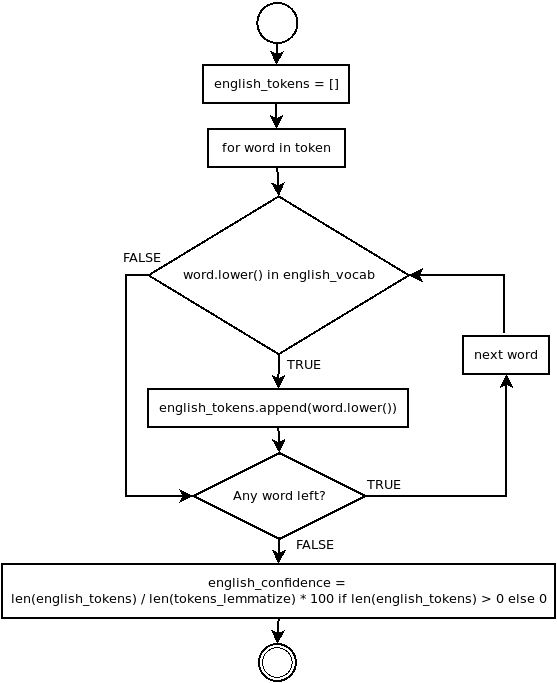
\includegraphics[width=0.65\textwidth]{Pictures/detect_lang.png}
    \caption{\label{fig:detect_lang}{} An algorithm for creating words list }
\end{figure}




Pseudo algorithm for website language determination process:
\begin{enumerate}
    \item A list which would contain all english words is initiated
    \item Each word from website tokens list is iterated
    \item If word appears in the english words dictionary, then word is appended to the english words list(step 1)
    \item Steps 1, 2, 3 are repeated until all words from the token list are iterated
    \item The ratio of english words in the website is calculated by dividing number of english words to total number words in the website token and multiplying by 100 to get percentage representation
    \item If the ratio is less then 50 \% and webpage contains less than 10 english words, then the website considered to be non english content and it would be excluded from the website list
\end{enumerate}
English words which was appended into english words list in step 1 is considered as new words token representation for website since all non english words are excluded.

English websites consist of 101 different top-level domains(TLD). The diversity of the 10 most frequent domains could be seen from the figure(\ref{fig:domain_diversity}) :

\begin{figure}[H]
    \centering
    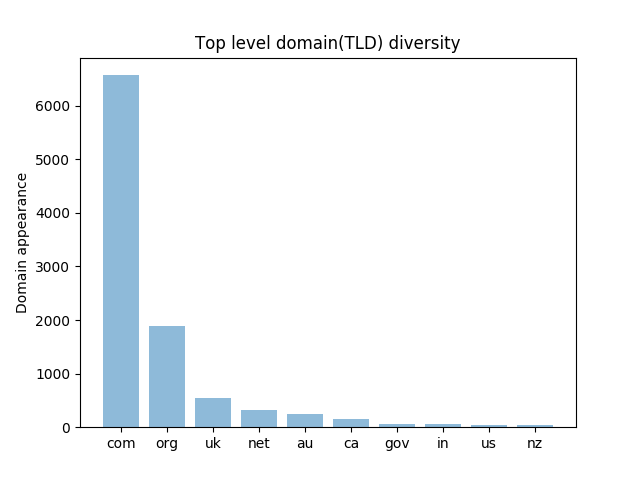
\includegraphics[width=1\textwidth]{Pictures/domain_diversity.png}
    \caption{\label{fig:domain_diversity}{}Top Level Domain(TLD) diversity in the english content websites}
\end{figure}

According to the generated results of TLD diversity in the english content websites (\ref{fig:domain_diversity}) the most frequent domain is \textbf{com} with \textit{6571} instances, the second place took \textbf{org} domain with \textit{1885} instances and the third place took \textbf{uk} domain with \textit{540} instances.

\subsubsection{Words list creation}

In theory every category should contain a different set of words that could represent category itself. At this point a new generated english words token list from the previous subsection contains words for particular website, but not for particular category. One website data is not enough to define the list of the most frequent words in a category, but all websites data are able to create a total word list of all websites for each category where the most frequent words list will be generated after all websites would be analyzed.

The total words list for 24 categories is generated by appending each website words from token list. The dictionary data type is created with shape of \textit{(24, x)} where first dimension represents the name of category and the second dimension represents the set of total words for each category. The value of second dimension is equal x, because each category could contain different number of words. 


Implementation of the total words list creation could be seen in the code flowchart figure(\ref{fig:words_list_creation}):
\begin{figure}[H]
    \centering
    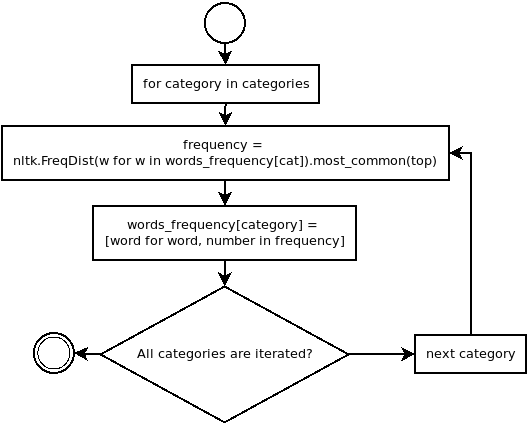
\includegraphics[width=1.05\textwidth]{Pictures/category_words_frequency.png}
    \caption{\label{fig:words_list_creation}{} An algorithm for creating words list }
\end{figure}

Total words list generation pseudo algorithm:
\begin{enumerate}
    \item Each category is iterated from the categories list
    \item If the dictionary do not have key instance of the current category, then dictionary with category key is initialized and it equals for empty list
    \item The dictionary list of category key is extended with a website words token list
    \item Step 1, 2, 3 is repeated until all categories are iterated
\end{enumerate}

Total words list for each category will take a place for creating a list of the most frequent words list for each category.


\subsection{Words frequency model}

This part would cover the most frequent word generation for each category. At this point, the words list should be generated from all websites words tokens including their categories. The words list contains all existing words for each category, so the main part of this section is to determine the most frequent words and sort them ascending mode. This list of the most frequent words would be used for the custom model prediction and also for features generation for Machine learning model.

This section consist of 2 parts:
\begin{enumerate}
    \item \textbf{The most frequently words list for categories} - a list of the most popular words list for each category
    \item \textbf{Chunk words} - methods for detecting chunk words and exclude them from the most frequent words list
\end{enumerate}


\subsubsection{The most frequently words list for categories}


All websites are classified into \hyperref[sec:categoriesSet]{24 categories}. Each category has it is own features which are defined by the words, for example: set of words ['World', 'Business', 'Science', 'Weather', 'Culture', ...] implies that it is probably a set of keywords that may belong to "News & Media" category. Humans could categorize websites content could classify intuitively if website keywords match well known patterns of the category.

The most frequent words list is made from the previously generated word list - all possible words for each category is stored into this list so the main task for this phase is to calculate the frequency of the words and sort them in ascending mode. The vector of the most frequent words list would consist of 2500 words for each category. 

The shape of the most frequent words list: \textit{(24, 2500)} in other words: \textit{categories list, 2500 the most frequent words)}. It is possible to have lower shape of the most frequent words if category all websites contains less then 2500 different words in that case number would be equal a set of words available in a category websites contents.


Implementation of the most frequently words list for categories creation could be seen in the code flowchart figure(\ref{fig:category_words_frequency}):
\begin{figure}[H]
    \centering
    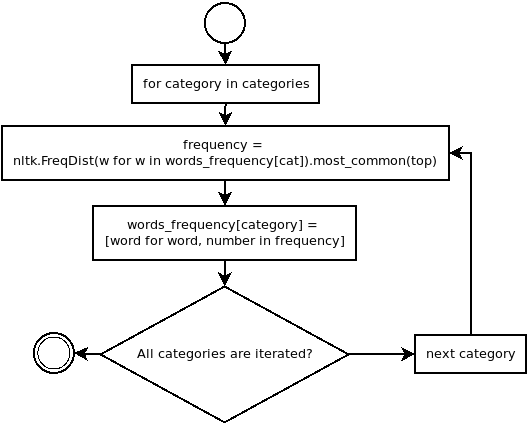
\includegraphics[width=1\textwidth]{Pictures/category_words_frequency.png}
    \caption{\label{fig:category_words_frequency}{} An algorithm for creating the most frequent words list for each category }
\end{figure}

The pseudo algorithm how the most frequent words list is made:
\begin{enumerate}
    \item Each category is iterated from the categories list
    \item Calculating words frequency for each category. The frequency is calculated by using \href{http://www.nltk.org/api/nltk.html?highlight=freqdist}{nltk.FreqDist} function. A function requires a string data type as parameter and it returns the tuple data type of words and their frequency occurrence. The input of the function is words list for each category. Each word from the words list is iterated and passed to the function. In this way the function returns word with it frequency. The words and frequency is sorted in ascending mode. Example of an output of TOP 5 most frequent words in 'Books\_and\_Literature category': $[('book', 5625), ('text', 4094), ('new', 2322), ('novel', 2009)...]$.
    \item Extracting words from the frequent words list. Since the only goal of this process is to generate a list of the most frequent words in the category, the number of words frequency would not be used for the Machine Learning model so only words are extracted and saved in the words frequency list.
\end{enumerate}


\subsubsection{Chunk words}

Generated words frequency list is not perfect because websites could contain a lot of chunk words which are common to all categories. Content of the websites could depend on many factors - current month, political news, casual news or default HTML home page design which includes words like contact or home. Words that are in the TOP 15 the most frequent word list and appears more or equal than 7 categories are called chunk words. 


Implementation of creating and removing chunk words could be seen in the code flowchart figure(\ref{fig:chunk_words}):
\begin{figure}[H]
    \centering
    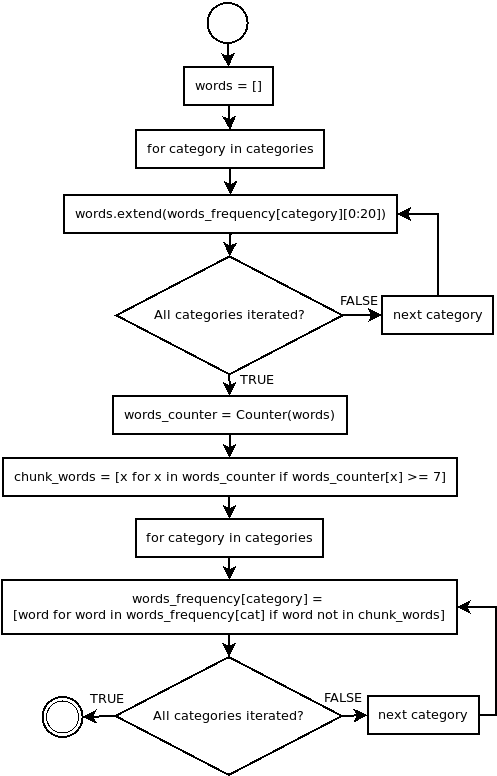
\includegraphics[width=0.65\textwidth]{Pictures/chunk_words.png}
    \caption{\label{fig:chunk_words}{}An algorithm for detecting and removing chunk words }
\end{figure}


The pseudo algorithm for detection of chunk words and chunk words removing process:
\begin{enumerate}
    \item An empty list \textit{words} is created where all top 15 words would be stored
    \item Each category is iterated from the categories list
    \item Top 15 most frequent words in each category is extended to the words list (Step 1)
    \item Steps 2 and 3 are repeated until all categories would be iterated
    \item Words are counted by using \href{https://docs.python.org/2/library/collections.html}{Counter} function
    \item If word appears more or equal than 7 times in different categories, then word is added to the chunk words list
    \item Each category is iterated from the categories list
    \item Words are excluded from the most frequent words list for category by checking if word is in the chunk words list
\end{enumerate}


All chunk words could be seen in the figure(\ref{fig:words_diversity}) :
\begin{figure}[H]
    \centering
    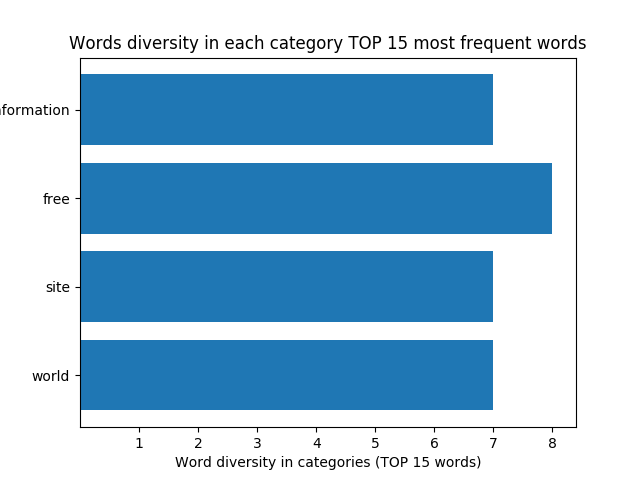
\includegraphics[width=1\textwidth]{Pictures/words_diversity.png}
    \caption{\label{fig:words_diversity}{}An diagram of chunk words diversity in categories }
\end{figure}


According from the most frequent words from each category data generated in December, the bar chart figure(\ref{fig:words_diversity}) shows that there are 4 chunks words: \textit{information, free, site, world}. The word 'free' appeared in a 8 categories while other words appeared in 7 categories. These words are excluded from the most frequent words list.

\subsection{Custom model}

Machine Learning approach is not only way to predict category of the website - other way is to use raw statistics and create a prediction model from already generated words frequency list of each category which was created in the previous section. Since it is known categories most popular words it is possible to find a pattern and predict a category of URL without Machine Learning approach. Custom model creation requires 2 steps:
\begin{enumerate}
    \item Categories features generation
    \item Calculate words weight
\end{enumerate}

This method do not require machine learning approach and it is capable of predicting category of the target website (a website which category will be predicted). Method performance results are much better than usual Machine Learning model. The results and conclusions of custom model are described in the "Results and Conclusion settings" section.

\subsubsection{Categories features generation}

The most frequent words list for categories is used not only for Machine Learning, but also for categories features generation. The method requires a \textit{target website most frequent word list} and \textit{categories most frequent words list} in order to generate the categories features list to determine a target website category. 


The first step of the model creation is gathering the most frequent word list of a target website. The main goal of this process is to create a most frequent words model for each category. Each category would have a list of words that occurred in the target website. At the beginning, each word in the list is equal to the value of 0. By going through each category, if the word occurs in the most frequent words list, then that position the value changes from 0 to 1.

The idea behind this process is to generate vector with the shape: \textbf{(categories number, number of top words in category)}. In implementation part there are  24 different categories and there are tracked top 2500 the most frequent words, so the shape of the list should be: \textbf{(24, 2500)} if there are no chunk words excluded, otherwise it would depend on the particular category most frequent words list length. 

Implementation of this process could be seen in the code flowchart figure(\ref{fig:category_features}):
\begin{figure}[H]
    \centering
    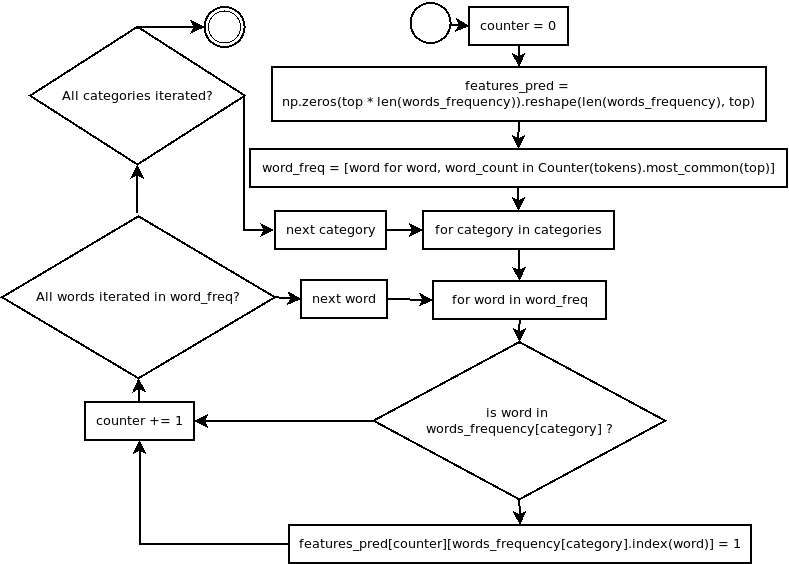
\includegraphics[width=0.9\textwidth]{Pictures/category_features.png}
    \caption{\label{fig:category_features}{}Algorithm of creating the most frequent word vector }
\end{figure}

The Categories features generation for the website pseudo algorithm:
\begin{enumerate}
    \item Creating integer variable "counter" which would track a category index of the list. At the beginning "counter" variable value is equal to 0
    \item Creating a list of the most frequent words: "frequent\_pred". Later on this variable would store of all possible combinations of each category of the most frequent words list.
    
    For each category values of the list are set to 0. 
    
    Variable shape: (25, 2500). First dimension of the list marks category, second dimension of the list marks the top 2500 most frequent words.
    
    \item Storing top 2500 the most frequent words in the "words\_freq" variable. The website all words are counter and sorted in the ascending order from the most frequent word to the least frequent word of top 2500 words. 
    \item Iterating for each category from the categories list
    \item Iterating for each word from the "words\_freq" variable
    \item Checking if the current category most frequent words list contains website current word. If it contains, the index of the word position in the words\_frequency list for current category is saved and used by changing a value of features\_pred[counter][index] from 0 to 1
    \item Step 4 repeats until there no unchecked words left in the word\_freq list
    \item Counter value is auto incremented by 1. This action means that the category is changed to the next one
    \item All steps above are repeated until all categories from the categories list are iterated
\end{enumerate}


In the result of this process the list of the most frequent website words for each category is created. At the beginning the vector is filled with 0 values, but if the word of the website occurs in the category top frequent words list, then the value at the particular position is changed to 1.


In the end of this process, the list of frequent words features is generated for each category. The website words have an impact of a list values. This process generates a list of possible features for each category so the next step is for deciding which feature suits model the best and it is first dimension value would be considered of a target website category.



\subsubsection{Categories weight estimation}


Model feature list which was generated in the previous section should be evaluated in order to extract the category of the target website. The feature estimation is done by processing weight calculation of each category of model feature list and then choosing the max value of the calculated categories which would be considered as category of the target website.


The weight estimation of the model feature list is done by iterating each category list and checking the position whenever values are equal to 1. Every position should have their own weight, because the word frequency list is sorted in ascending mode so words that are close to the list beginning should be more important than those words that are near list end. The main formula of calculating weights of each category is: 
\begin{equation}
    weight\_sum = top - index
\end{equation}
\begin{description}
    \item [weight\_sum] A total sum of all words weights in the category
    \item [top] is a value of how much words are in the most frequent words list which by default value is equal to 2500
    \item [index] An index of where the value of 1 occurred in the category features list
\end{description}


The process of category weight estimation flowchart could be seen in the figure(\ref{fig:category_weight_estimation}):
\begin{figure}[H]
    \centering
    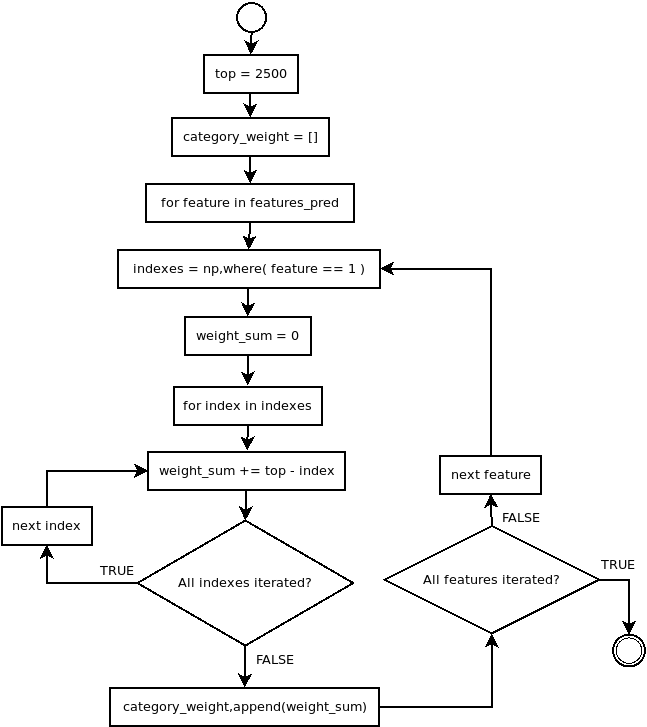
\includegraphics[width=0.85\textwidth]{Pictures/category_weight_estimation.png}
    \caption{\label{fig:category_weight_estimation}{} An algorithm of categories features weight estimation process}
\end{figure}


Category weight estimation pseudo algorithm:


\begin{enumerate}
    \item Creating a list where each category weight sum would be stored. The list is named as \textit{category\_weight}
    \item Iterating for each category features from the categories features list
    \item Getting all positions of the category features list where value is equal to 1. This is done by using \hyperref{https://docs.scipy.org/doc/numpy-1.15.0/reference/generated/numpy.where.html}{np.where()} function. This function requires an input of condition and it generated the position indexes as an output. The condition as an argument to the \hyperref{https://docs.scipy.org/doc/numpy-1.15.0/reference/generated/numpy.where.html}{np.where()} function: $category\_feature == 1$. The function iterates each value of the category features list and if that value is equal to 1, then it stores that value index in the category features list. The output of the function is stored to the \textit{indexes} variable as a numpy data list type.
    \item Creating an integer type variable for storing weight sums for category features list. The variable is named as \textit{weight\_sum}. At the start this variable value is equal to 0
    \item Iterating for each index of \textit{indexes} numpy list
    \item Calculating a weight sum for category features: $weight\_sum += top - index$
    \item Step 6 is repeated until all indexes are iterated
    \item The category features weight is appended into \textit{category\_weigh} list
    \item Steps 2, 3, 4 ,5, 6, 7, 8 are repeated until all categories features are iterated
\end{enumerate}


The main point of this process is to generate a list of all weights for each category features. That list is named as \textit{category\_weight}. At this point the main task is to track the category from the categories features list of the highest weight sum by using \hyperref{https://docs.python.org/3/library/functions.html}{max()} function which returns the highest value in the list. As an input function requires a list and as an output it returns the highest value in the input list. The output value of the highest category features weight sum is indicating website category by using \hyperref{https://docs.python.org/3/library/array.html#array.array.index}{index()} function which returns the index of the input value: $category\_index = category\_weight.index(max(category\_weight))$





\subsection{Machine Learning}


In this section Machine learning algorithms would be trained and tested using by already created the most frequent words list for categories, websites words data and websites categories. The main point of this section is to create a fully working Machine Learning model which would be able to predict a website category without no human interaction for the primary data set.

This is done by processing 4 steps:
\begin{enumerate}
    \item Features and labels creation
    \item Machine Learning models training
    \item Models performance evaluation
\end{enumerate}

\subsubsection{Features and labels creation}

Machine learning algorithms models requires a proper form of data which is the main key of the successful performance of Machine Learning models. At this point the data is almost set up properly - the most frequent words list for categories is created which would help in creating a features and labels for Machine Learning model. Features and labels definitions:
\begin{description}
    \item [Features] are attributes or properties shared by all of the independent units on which analysis or prediction is to be done. 
    
    In this project the features would be considered to be binarized websites most frequent words lists according to the most frequent words list for category list. If a target website most frequent words list values are in the most frequent words list for specific category list, then the value in the most frequent website words list is changed 1 in a position of a word, otherwise value is set to 0.
    
    
    Data set contains the categories of all websites, so in this case it is known which category of the most frequent words list for categories has to be used. 
    \item [Labels] are the final output.
    
    In this project labels are the categories of websites. Since the data set contains all categories of websites so the main task is to track them properly and match them with the features that Machine Learning model would know category of particular website feature set.
\end{description}


The process of features and labels creation for Machine Learning model flowchart could be seen in the figure(\ref{fig:features_labels_creation}):
\begin{figure}[H]
    \centering
    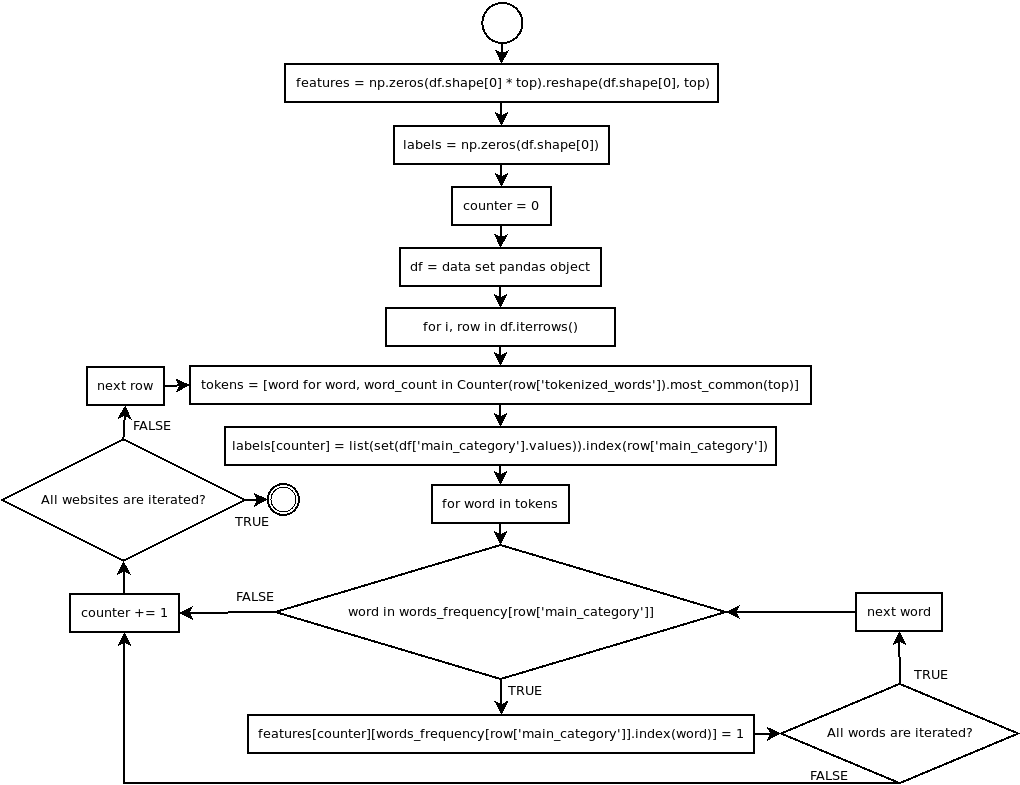
\includegraphics[width=1.085\textwidth]{Pictures/features_labels_creation.png}
    \caption{\label{fig:features_labels_creation}{} An algorithm of features and labels creation}
\end{figure}


Features and labels creation pseudo algorithm:
\begin{enumerate}
    \item List named \textit{features} is created for storing websites features. The features list has a shape of \textbf{(english website length in the data set, top)} which is equals to \textbf{(10436, 2500)} by using december websites data set.
    \item List named \textit{labels} is created for storing websites labels. The labels list has 1-dimensional shape of \textbf{(english website length in the data set)} which is equals to \textbf{(10436)} by using december websites data set.
    \item Integer variable \textit{counter} is created for tracking an index of \textit{labels} list and 1-dimension of \textit{features} list. At the beginning this variable is set to be equal 0
    \item Iterating for each website(\textit{row}) and their position(\textit{i}) in the december websites data set
    \item Defining \textit{labels} list value in the position of \textit{counter}. The category of the website is saved into \textit{labels} list of \textit{counter} position
    \item Iterating for \textit{word} in website token list
    \item Checking if \textit{word} is in the most frequent words list for the current category - if it is true, then \textit{features} list value in 1-dimensional position of \textit{counter} and 2-dimensional position of word in the most frequent words list for current category is set to 1
    \item Steps 7 is repeated until all words are iterated from a website token list
    \item \textit{counter} value is auto incremented by 1
    \item Steps 5, 6, 7, 8, 9 are repeated until all websites are iterated from the december websites data set 
\end{enumerate}


Features and labels are the main data that would be fit to Machine Learning models. However it is a bad practise to use all this data on training machine learning models because of these factors:
\begin{enumerate}
    \item Testing machine learning model. If all data would be used for machine learning model training, then how to be sure how well the model is performing in predicting data set if there are no testing data? Testing data is an indicator of how well machine learning model is performing.
    \item Over fitting problem. Over fit is when your training model is too precise and doesn't generalize on the problem you try to solve. In other words it is too fit for the training, and the training alone, so that it cannot solve/predict a different data set. 
\end{enumerate}

These factors are the reason why features and labels data should be split into \textbf{training} data and \textbf{testing} data. 

At first features and labels data are shuffled by using \href{https://scikit-learn.org/stable/modules/generated/sklearn.utils.shuffle.html}{sklearn.utils.shuffle(*arrays, **options)} function. It shuffles arrays or sparse matrices in a consistent way. Function main argument is features and labels data sets which should be shuffled.


The next step of the shuffled data create training and testing data sets by using \href{https://scikit-learn.org/stable/modules/generated/sklearn.model_selection.train_test_split.html}{sklearn.model_selection.train_test_split(*arrays, **options)} function. This function splits arrays or matrices into random train and test subsets by proportion of 67 \% of total data to training data, and 33 \% of remaining data to the testing data.  


\subsubsection{Machine learning models creation}


Building machine learning models from the scratch requires a lot of time and advanced knowledge about concepts of a particular machine learning model parameters implementations. Machine learning models for implementation part would be created by using Machine learning libraries where a lot of models are already build in. Models are created by using \href{https://scikit-learn.org/stable/}{scikit-learn}  library for python programming language. scikit-learn python library has build in already prepared ready to use machine learning models.


In the implementation part there are created 2 different approach supervised machine learning classifiers types:
\begin{enumerate}
    \item \textbf{Logistic Regression (LR)}
    
    Logistic regression model is created by using \hyperref{https://scikit-learn.org/stable/modules/generated/sklearn.linear_model.LinearRegression.html}{sklearn.linear_model.LinearRegression} library. Fundamentals of the Logistic Regression model are described in the Logistic regression section(\ref{sssec:logistic_regression})
    
    \item \textbf{Linear Support Vector Classification (LSVC)}
    
    Linear Support Vector Classification is one of the branch of Support Vector Machine (SVM) classification model in other words - they are different implementation of the same algorithm. 
    
    The difference between LSVC and SVM: A regular SVM with default values uses a radial basis function as the SVM kernel while LSVC uses a linear kernel for the basis function. That makes LSVC model much less tunable and is basically just a linear interpolation.
    
    Linear Support Vector Classification is created by using \hyperref{https://scikit-learn.org/stable/modules/generated/sklearn.svm.LinearSVC.html}{sklearn.svm.LinearSVC} library with default parameters. LSVC parameters are almost identical as Logistic regression model, except:
\end{enumerate}

Each model has their properties that would have an impact to the model performance. In Logistic Regression and Linear Support Vector Classification shares almost identical parameters. Some of the models parameters description:
\begin{itemize}
    \item \textit{C = 1.0}. C parameter is inverse of regularization strength. Smaller values of C specify stronger regularization. This variable value must be positive. C value is set to 1.0
    \item \textit{class\_weight = None}. Weights associated with classes in the form \{class\_label: weight\}. This value is set up to 'None', because all classes supposed to have at least one weight
    \item \textit{penalty = 'l2'}. Used to specify the norm used in the penalization. L2 penalty indicates that model uses \textit{Ridge Regression} regularization technique.
    \item \textit{dual}. Dual or primal formulation. Dual formulation is only implemented for l2 penalty with liblinear solver. Prefer dual = False when n\_samples > n\_features. In \textbf{Logistic Regression} model dual parameter is set to False, while in \textbf{Linear Support Vector Classification} model dual parameter is set to True.
    \item \itemit{Fit\_intercept = True}. The intercept is the expected mean value of features when all labels are equal to constant value.
    \item \itemit{intercept\_scaling = 1}. Intercept scaling is used to lessen the effect of regularization on synthetic feature weight.
    \item \itemit{max\_iter = 100}. Maximum number of iterations taken for the solvers to converge.
    \item \itemit{random\_state = None}. The seed of the pseudo random number generator to use when shuffling the data
    \item \itemit{tol = 0.0001}. Tolerance for stopping criteria
    \item \itemit{warm\_start = False}. When set to True, reuse the solution of the previous call to fit as initialization, otherwise, just erase the previous solution
\end{itemize}


The last step is to train created Machine Learning models in order to classify websites. This is done by passing generated training features set and training labels set to the \href{https://scikit-learn.org/stable/modules/generated/sklearn.linear_model.LinearRegression.html}{fit method}. Fitting models to the training data is essentially the training part of the modeling process. It finds the coefficients for the equation specified via the algorithm being used. 

Machine learning models after fitting procedure could predict category of the website. The results of prediction may concern of how well data was prepared and also what kind of Machine Learning algorithm was chosen. The prediction is done by using \href{https://scikit-learn.org/stable/tutorial/statistical_inference/supervised_learning.html}{Supervised learning predict function}. This function input is test features set and it returns a labels set of a given features. 

\subsubsection{Models performance evaluation}

Models performance evaluation score is a result of how well models are trained. Evaluation process is performed using 2 different data sets with different websites list. First data set is the original data set from where training/testing features/labels set were created. Second data set is custom made which contains english language websites links with labeled categories.

\begin{enumerate}
    \item \textbf{Models performance evaluation using original data set}.
    
    Primary data set allows evaluate performance for three different parameters: \textif{Precision score, Recall score and F1-score}. Scores evaluations are made for 2 models: Linear Regression model and Linear Support Vector Machine model. 
    
    Since models solves multi-class machine learning approach, because labels consist of 25 different categories, evaluations methods are applied on each category.
    
    \pagebreak
    \textbf{Logistic Regression} model prediction evaluation analysis:

    \begin{table}[H]
        \centering
        \begin{tabular}{l|c|c|c|}
            \hline
            \multicolumn{1}{c}{}  & \multicolumn{3}{|c|}{Logistic Regression}\\\cline{2-4}
            \textbf{Category} & \multicolumn{1}{l|}{\textbf{precision}} & \multicolumn{1}{l|}{\textbf{recall}} & \multicolumn{1}{l|}{\textbf{f1-score}} \\ \hline
            Recreation\_and\_Hobbies & 0.98 & 0.86 & 0.91 \\ \cline{2-4} 
            Food\_and\_Drink & 0.84 & 0.86 & 0.85 \\ \cline{2-4} 
            News\_and\_Media &  0.86 & 0.92 & 0.89  \\ \cline{2-4} 
            Travel & 0.87 & 0.66 & 0.75  \\ \cline{2-4} 
            Career\_and\_Education & 0.93 & 0.80 & 0.86 \\ \cline{2-4} 
            Home\_and\_Garden & 0.88 & 0.86 & 0.87 \\ \cline{2-4} 
            Internet\_and\_Telecom & 0.87 & 0.81 & 0.84 \\ \cline{2-4} 
            Gambling & 0.80 & 0.90 & 0.85 \\ \cline{2-4} 
            Books\_and\_Literature & 0.87 & 0.95 & 0.91 \\ \cline{2-4} 
            Science & 0.95 & 0.88 & 0.91 \\ \cline{2-4} 
            Health & 0.82 & 0.59 & 0.69  \\ \cline{2-4} 
            Autos\_and\_Vehicles & 0.94 & 0.89 & 0.92 \\ \cline{2-4} 
            Finance & 0.80 & 0.86 & 0.83 \\ \cline{2-4} 
            Sports &  0.87 & 0.85 & 0.86 \\ \cline{2-4} 
            Adult & 0.81 & 0.83 & 0.82 \\ \cline{2-4} 
            Pets\_and\_Animals & 0.92 & 0.90 & 0.91 \\ \cline{2-4} 
            Business\_and\_Industry & 0.80 & 0.90 & 0.85 \\ \cline{2-4} 
            People\_and\_Society & 0.83 & 0.26 & 0.40 \\ \cline{2-4} 
            Law\_and\_Government & 0.89 & 0.87 & 0.88 \\ \cline{2-4} 
            Beauty\_and\_Fitness & 0.94 & 0.91 & 0.93 \\ \cline{2-4} 
            Arts\_and\_Entertainment & 0.76 & 0.79 & 0.78 \\ \cline{2-4} 
            Games & 0.88 & 0.81 & 0.84 \\ \cline{2-4} 
            Reference & 0.85 & 0.76 & 0.80 \\ \cline{2-4} 
            Computer\_and\_Electronics & 0.25 & 0.11 & 0.15 \\ \cline{2-4} 
            Shopping &  0.94 & 0.85 & 0.89 \\ \cline{2-4} 
        \end{tabular}
        \caption{Logistic regression model performance evaluation for each category}
        \label{table: lr_table}
    \end{table}
    
    Logistic regression model evaluation scores table (\ref{table: lr_table}) indicates that the most positive predictions (\textit{precision score}) model made on "Recreation\_and\_Hobbies" category with \textbf{0.98 precision score}; category of the highest actual positives identification proportion (\textit{recall score}) is "Books\_and\_Literature" with  \textbf{0.95 recall score}; category of the highest harmonic mean of precision and recall scores is "Beauty\_and\_Fitness" with  \textbf{0.93 f1 score}.
    
    Logistic Regression model overall mean scores for all categories:
    \label{sssec:lr_overall}
    \begin{itemize}
        \item Accuracy score:  0.85
        \item Precision score: 0.85
        \item Recall score: 0.79
        \item F1 score: 0.81
    \end{itemize}
    
    
    Logistic Regression model confusion matrix heat map for each category (\ref{fig:lr_confusion_matrix}):
    \begin{figure}[H]
        \centering
        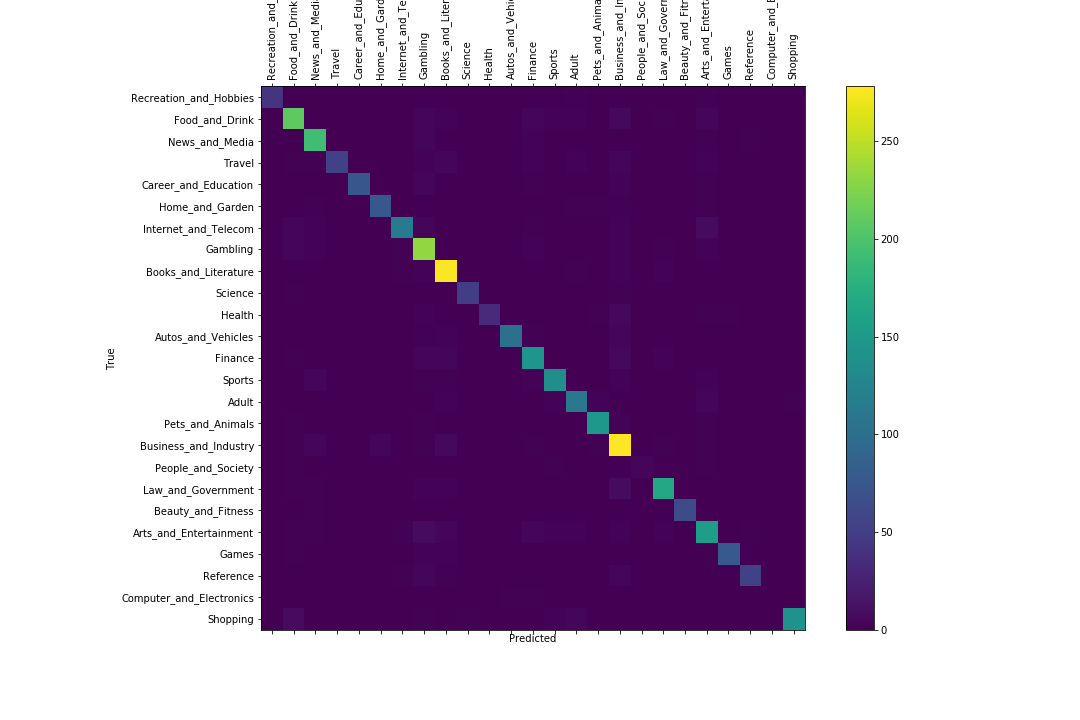
\includegraphics[width=1.2\textwidth]{Pictures/lr_confusion_matrix.png}
        \caption{\label{fig:lr_confusion_matrix}{} Confusion matrix of Logistic Regression model}
    \end{figure}
    
    \pagebreak
    \textbf{Linear Support Vector Machine} model prediction evaluation analysis:
    
    \begin{table}[H]
        \centering
        \begin{tabular}{l|c|c|c|}
            \hline
            \multicolumn{1}{c}{}  & \multicolumn{3}{|c|}{Linear Support Vector Machine}\\\cline{2-4}
            \textbf{Category} & \multicolumn{1}{l|}{\textbf{precision}} & \multicolumn{1}{l|}{\textbf{recall}} & \multicolumn{1}{l|}{\textbf{f1-score}} \\ \hline
            Recreation\_and\_Hobbies & 0.78 & 0.80 & 0.79 \\ \cline{2-4} 
            Food\_and\_Drink &  0.81 & 0.78 & 0.79\\ \cline{2-4} 
            News\_and\_Media &  0.81 & 0.87 & 0.84  \\ \cline{2-4} 
            Travel & 0.79 & 0.54 & 0.64  \\ \cline{2-4} 
            Career\_and\_Education & 0.83 & 0.72 & 0.77 \\ \cline{2-4} 
            Home\_and\_Garden & 0.79 & 0.84 & 0.8 \\ \cline{2-4} 
            Internet\_and\_Telecom & 0.76 & 0.72 & 0.74 \\ \cline{2-4} 
            Gambling & 0.76 & 0.83 & 0.79 \\ \cline{2-4} 
            Books\_and\_Literature & 0.86 & 0.88 & 0.87  \\ \cline{2-4} 
            Science & 0.86 & 0.86 & 0.86 \\ \cline{2-4} 
            Health & 0.62 & 0.52 & 0.56 \\ \cline{2-4} 
            Autos\_and\_Vehicles & 0.86 & 0.84 & 0.85 \\ \cline{2-4} 
            Finance & 0.76 & 0.78 & 0.77 \\ \cline{2-4} 
            Sports &  0.73 & 0.75 & 0.74 \\ \cline{2-4} 
            Adult & 0.77 & 0.75 & 0.76 \\ \cline{2-4} 
            Pets\_and\_Animals & 0.88 & 0.88 & 0.88 \\ \cline{2-4} 
            Business\_and\_Industry & 0.79 & 0.85 & 0.82 \\ \cline{2-4} 
            People\_and\_Society & 0.36 & 0.21 & 0.27 \\ \cline{2-4} 
            Law\_and\_Government & 0.82 & 0.82 & 0.82 \\ \cline{2-4} 
            Beauty\_and\_Fitness & 0.86 & 0.78 & 0.82  \\ \cline{2-4} 
            Arts\_and\_Entertainment & 0.72 & 0.74 & 0.73 \\ \cline{2-4} 
            Games & 0.71 & 0.73 & 0.72  \\ \cline{2-4} 
            Reference &  0.75 & 0.65 & 0.70 \\ \cline{2-4} 
            Computer\_and\_Electronics &  0.08 & 0.11 & 0.09 \\ \cline{2-4} 
            Shopping &   0.81 & 0.77 & 0.79 \\ \cline{2-4} 
        \end{tabular}
        \caption{Linear support vector machine model performance evaluation for each category}
        \label{table: svm_table}
    \end{table}


     Linear support vector machine model evaluation scores table (\ref{table: lr_table}) indicates that the most positive predictions (\textit{precision score}) model made on "Pets\_and\_Animals" category with \textbf{0.88 precision score}; category of the highest actual positives identification proportion (\textit{recall score}) is "Books\_and\_Literature" and "Pets\_and\_Animals" with  \textbf{0.88 recall score}; category of the highest harmonic mean of precision and recall scores is "Pets\_and\_Animals" with  \textbf{0.88 f1 score}.
    
    Linear support vector machine model overall mean scores for all categories:
    \label{sssec:lsvm_overall}
    \begin{itemize}
        \item Accuracy score: 0.79
        \item Precision score: 0.74
        \item Recall score: 0.72
        \item F1 score: 0.73
    \end{itemize}
    
    
    Linear support vector machine model confusion matrix heat map for each category (\ref{fig:lsvm_confusion_matrix}):
    \begin{figure}[H]
        \centering
        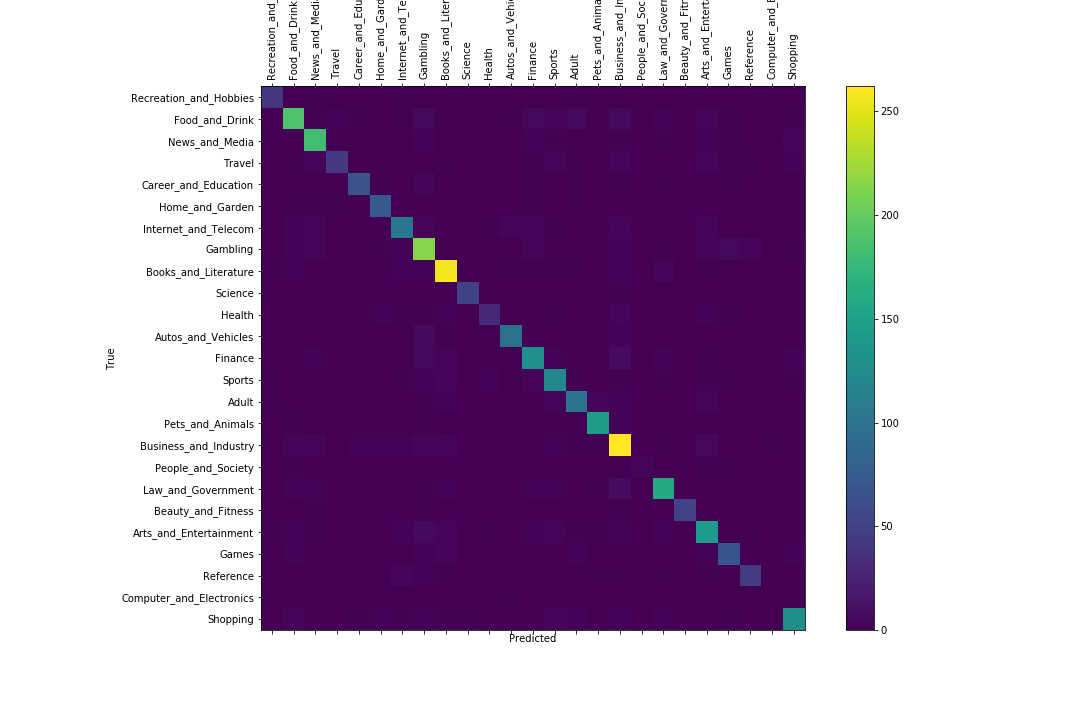
\includegraphics[width=1.2\textwidth]{Pictures/lsvm_confusion_matrix.png}
        \caption{\label{fig:lsvm_confusion_matrix}{} Confusion matrix of Linear Support Vector Machine model}
    \end{figure}
    
    
    Models performance overall evaluation (\ref{sssec:lr_overall}, \ref{sssec:lsvm_overall}) results  implies that model with the best performance for classifying websites categories is \textbf{Linear Regression} model. 
    
\item \textbf{Models performance evaluation using custom made data set}.

Original data set evaluation score is not an final indicator that machine learning models are performing well. The original data set has two serious flaws which could have an impact for final models results. 
\begin{enumerate}
    \item Data set could be outdated. The original data set is created in 2014 year so some of websites content could be changed or not working that leads to another problem that data set classified labels could be changed in the current time.
    \item Classified labels could be wrong. The original data set contains 31086 different websites so to check each website category would consume too much time. Revision of labeled websites would be great to make sure that declared category of particular website is correct
\end{enumerate}

These problems are solved by creating small custom made data set for testing performance on created machine learning models. The custom data set consist of 288 working english websites with human confirmed categories. Each website is iterated and content is download in the same manner of original data set.

On custom model data set is tested my created website categorization model \ref{custom_model} which predicts category of website by creating feature set for each category and calculating weight of the features set. The feature set with the highest weight is considered to be category of the website.

Performance evaluation using custom made data set on my custom model and machine learning models, testing on 286 different websites and there are performance results:

\begin{itemize}
    \item \textbf{Custom model}: 69.5 \% (197 correct predictions of 282)
    \item \textbf{Logistic regression model}: 57.8 \% (163 correct predictions of 282)
    \item \textbf{Linear support vector machine model}: 52.5 \% (148 correct predictions of 282)
\end{itemize}
From given results custom model performance is the best for predicting up to date websites categories. Machine learning models performance is similar - logistic regression manage correctly predict 163 websites categories while linear support vector machine 148 websites categories. According to original data set machine learning models results - linear regression model should perform better than linear support vector machine and that confirms performance results on the custom data set.

\pagebreak
Models performance on predicting each category:

 \begin{table}[H]
        \centering
        \begin{tabular}{l|c|c|c|}
            \hline
            \multicolumn{1}{c}{}  & \multicolumn{3}{|c|}{Custom data set performance evaluation}\\\cline{2-4}
            \textbf{Category} & \multicolumn{1}{l|}{\textbf{Custom model}} & \multicolumn{1}{l|}{\textbf{LR model}} & \multicolumn{1}{l|}{\textbf{LSVM model}} \\ \hline
            Food\_and\_Drink & 6 / 7 : 85.71 \% & 6 / 7 : 85.71 \% & 6 / 7 : 85.71 \% \\ \cline{2-4} 
            News\_and\_Media &  12 / 14 : 85.71 \% & 11 / 14 : 78.57 \% & 11 / 14 : 78.57 \%  \\ \cline{2-4} 
            Travel & 13 / 15 : 86.67 \% & 8 / 15 : 53.33 \% & 7 / 15 : 46.67 \%  \\ \cline{2-4} 
            Career\_and\_Education & 14 / 14 : 100.00 \% & 11 / 14 : 78.57 \% & 9 / 14 : 64.29 \% \\ \cline{2-4} 
            Home\_and\_Garden & 3 / 16 : 18.75 \% & 2 / 16 : 12.50 \% & 2 / 16 : 12.50 \% \\ \cline{2-4} 
            Internet\_and\_Telecom & 3 / 16 : 18.75 \% & 3 / 16 : 18.75 \% & 2 / 16 : 12.50 \% \\ \cline{2-4} 
            Gambling & 9 / 9 : 100.00 \% &  6 / 9 : 66.67 \% & 5 / 9 : 55.56 \% \\ \cline{2-4} 
            Books\_and\_Literature & 7 / 10 : 70.00 \% & 7 / 10 : 70.00 \% & 7 / 10 : 70.00 \% \\ \cline{2-4} 
            Science & 16 / 20 : 80.00 \% & 13 / 20 : 65.00 \% & 11 / 20 : 55.00 \% \\ \cline{2-4} 
            Health & 9 / 11 : 81.82 \% & 6 / 11 : 54.55 \% & 6 / 11 : 54.55 \%  \\ \cline{2-4} 
            Autos\_and\_Vehicles & 13 / 16 : 81.25 \% & 13 / 16 : 81.25 \% & 12 / 16 : 75.00 \% \\ \cline{2-4} 
            Finance & 13 / 19 : 68.42 \% & 12 / 19 : 63.16 \% & 12 / 19 : 63.16 \% \\ \cline{2-4} 
            Sports & 8 / 9 : 88.89 \% & 7 / 9 : 77.78 \% & 5 / 9 : 55.56 \% \\ \cline{2-4} 
            Adult & 8 / 8 : 100.00 \% & 7 / 8 : 87.50 \% & 5 / 8 : 62.50 \% \\ \cline{2-4} 
            Pets\_and\_Animals & 9 / 12 : 75.00 \% & 5 / 12 : 41.67 \% & 5 / 12 : 41.67 \% \\ \cline{2-4} 
            Business\_and\_Industry & 4 / 8 : 50.00 \% & 3 / 8 : 37.50 \% & 3 / 8 : 37.50 \% \\ \cline{2-4} 
            People\_and\_Society & 1 / 1 : 100.00 \% & 1 / 1 : 100.00 \% & 1 / 1 : 100.00 \% \\ \cline{2-4} 
            Law\_and\_Government & 6 / 8 : 75.00 \% & 4 / 8 : 50.00 \% & 4 / 8 : 50.00 \% \\ \cline{2-4} 
            Beauty\_and\_Fitness & 19 / 23 : 82.61 \% & 16 / 23 : 69.57 \% & 14 / 23 : 60.87 \% \\ \cline{2-4} 
            Arts\_and\_Entertainment & 2 / 10 : 20.00 \% & 2 / 10 : 20.00 \% & 2 / 10 : 20.00 \% \\ \cline{2-4} 
            Games & 3 / 6 : 50.00 \% & 2 / 6 : 33.33 \% & 2 / 6 : 33.33 \% \\ \cline{2-4} 
            Reference & 1 / 10 : 10.00 \% & 1 / 10 : 10.00 \% & 1 / 10 : 10.00 \% \\ \cline{2-4} 
            Computer\_and\_Electronics & 12 / 13 : 92.31 \% & 12 / 13 : 92.31 \% & 12 / 13 : 92.31 \% \\ \cline{2-4} 
            Shopping &  6 / 7 : 85.71 \% & 5 / 7 : 71.43 \% & 4 / 7 : 57.14 \% \\ \cline{2-4} 
        \end{tabular}
        \caption{Models performance on predicting each category}
        \label{table: custom_table}
    \end{table}
\end{enumerate}

According to the custom data set performance results(\ref{table: custom_table}) models performance on predicting category the best results are performed on category "Career\_and\_Education" where custom model predicts of 100 \% accuracy; logistic regression model and linear support vector machine model predict on 78.57 \% accuracy. Not all predictions on categories are equal, because there are different websites instances of categories. For example: category "People\_and\_Society" all models predicted at 100 \% accuracy, but this is not quite accurate since there is only 1 website with in the custom data set with that category. To make this evaluation more accurate, the custom data set should be expanded with more websites instances and websites instances on categories number should be equal for all categories.  



 %Conclusions section
\sectionWithoutNumber{\keyWordConclusions}{conclusion}

All created models accuracy on predicting real world websites categories are greater than 50 \%. Statistically that models most likely should have more correct predictions than incorrect in a long term.

During implementation part there was created 3 models which are capable of classifying websites:
\begin{enumerate}
    \item \textbf{Custom model}
    \item \textbf{Logistic Regression model}
    \item \textbf{Linear Support Vector Machine model}
\end{enumerate}


There are 2 websites data sets with websites URL's and categories:
\begin{enumerate}
    \item \textbf{Original data set}
    
    Original data set is an open source and it is available at \href{https://www.figure-eight.com/data-for-everyone/}{Data For Everyone data set lists}. The data set contains 31086 different URLs with 81 attributes. 
    
    This data set is used to create \textit{the most frequent words list for categories} and \textit{training/testing features and labels sets} for machine learning models.
    
    
    Machine learning performance on the original data set features set:
    \begin{enumerate}
        \item \textbf{Logistic Regression}
        
            \begin{itemize}
                \item Accuracy score: 0.85
                \item Precision score: 0.85
                \item Recall score: 0.79 
                \item F1 score: 0.81
            \end{itemize}
        
        \item \textbf{Linear Support Vector Machine}
        
            \begin{itemize}
                    \item Accuracy score: 0.79
                    \item Precision score: 0.74
                    \item Recall score: 0.72
                    \item F1 score: 0.73
            \end{itemize}
            
    \end{enumerate}
    \item Custom data set
    
    Custom data set is human made website data set with 282 differently labeled websites. 
    
    Models accuracy performance on the custom data set:
    
    \begin{enumerate}
        \item \textbf{Custom model}: 69.5 \% (197 correct predictions of 282 websites)
        \item \textbf{Logistic Regression}: 57.8 \% (163 correct predictions of 282 websites)
        \item \textbf{Linear Support Vector Machine}: 52.5 \% (148 correct predictions of 282 websites)
    \end{enumerate}
\end{enumerate}

List of methods that would improve project results:

\begin{itemize}
    \item \textbf{Download content of website recursively}.
    
    This would take a lot of time but may improve the most words frequency list for categories generation since all links in the website would be visited and all information would be scraped. 
    
    At this project just one website home page is scraped and it takes about 23 hours to analyse all websites from the original data sets. Scraping all website links would take much more time but it would be more efficient
    
    \item \textbf{Revise website categories in the original data set}. 
    
    Original data set contains 31086 instances of labeled websites. However the data set was created in 2014 year so it is possible that websites content is changed and the category is also changed according to the website content. The solution would be to have human validation on website categories to confirm if declared category match the reality and is valid.
    
    \item \textbf{Translate non english content websites to english language}.
    
    Models are capable to predict categories for those websites which the language of content is english. This is the problem because the number of websites is reduced since there are a lot of websites with non english content. In the original data set after filtering out non english websites the number of websites instances reduced from 31086 websites to 10436 websites. 
    
    The solution would be translate website non english content to the english language. However, at the moment only "Google" are offering translation API services but these services are with symbols and intensity restrictions which do not allow properly translate websites.
    
    Translation implementation would allow models to predict any website with any language and automatically the variaty of websites would be much bigger.
    
    \item \textbf{Improve custom data set} .
    
    \begin{enumerate}
        \item The custom data set should be expanded with more websites instances
        \item Websites instances on categories number should be equal for all categories. Some categories do not have any website or have just a few websites
    \end{enumerate}
    
    \item \textbf{Revise categories}. 
    
    Categories of websites sometimes could not be identified accurately since the website data could contain words that would cover multiple categories. Some categories are similar to other categories, for example: "Business\_and\_Industry" and "Finance" or "Internet\_and\_Telecom" and "People\_and\_Society". 
    
    For each category need to make an analysis to define main key words for particular category.

\end{itemize}


%ateities darbų gairės, planas/next steps of the work
% \sectionWithoutNumber{Ateities tyrimų planas}{future}{Pristatomi ateities darbai ir/ar jų planas, gairės tolimesniems darbams....}

 %file literatureSources.bib
\referenceSources{literatureSources}


\end{document}
